%% Settings for single-side (simplex) printing
% Margins: left 40mm, right 25mm, top and bottom 25mm
% (but beware, LaTeX adds 1in implicitly)
\documentclass[12pt,a4paper]{report}
\setlength\textwidth{145mm}
\setlength\textheight{247mm}
\setlength\oddsidemargin{7.5mm}
\setlength\evensidemargin{7.5mm}
\setlength\topmargin{0mm}
\setlength\headsep{0mm}
\setlength\headheight{0mm}
% \openright makes the following text appear on a right-hand page
\let\openright=\clearpage

%% Character encoding: usually latin2, cp1250 or utf8:
\usepackage[utf8]{inputenc}

%% Prefer Latin Modern fonts
\usepackage{lmodern}

\usepackage{amsmath}        % extensions for typesetting of math
\usepackage{amsfonts}       % math fonts
\usepackage{amsthm}         % theorems, definitions, etc.
\usepackage{bbding}         % various symbols (squares, asterisks, scissors, ...)
\usepackage{bm}             % boldface symbols (\bm)
\usepackage{graphicx}       % embedding of pictures
\usepackage{fancyvrb}       % improved verbatim environment
\usepackage{natbib}         % citation style AUTHOR (YEAR), or AUTHOR [NUMBER]
\usepackage[nottoc]{tocbibind} % makes sure that bibliography and the lists
			    % of figures/tables are included in the table
			    % of contents
\usepackage{dcolumn}        % improved alignment of table columns
\usepackage{booktabs}       % improved horizontal lines in tables
\usepackage{paralist}       % improved enumerate and itemize
\usepackage[usnames]{xcolor}  % typesetting in color
\usepackage{float}
\usepackage[boxruled]{algorithm2e}
\usepackage{gensymb}

\usepackage{listings}
\usepackage{color}

\definecolor{dkgreen}{rgb}{0,0.6,0}
\definecolor{gray}{rgb}{0.5,0.5,0.5}
\definecolor{mauve}{rgb}{0.58,0,0.82}

\lstset{frame=tb,
  language=Java,
  aboveskip=3mm,
  belowskip=3mm,
  showstringspaces=false,
  columns=flexible,
  basicstyle={\small\ttfamily},
  numbers=none,
  numberstyle=\tiny\color{gray},
  keywordstyle=\color{blue},
  commentstyle=\color{dkgreen},
  stringstyle=\color{mauve},
  breaklines=true,
  breakatwhitespace=true,
  tabsize=3
}

\usepackage{enumitem}
\usepackage{courier}
\usepackage{epstopdf}
\begin{document}

% TITLE PAGE
\begin{titlepage}
    \begin{center}
        \vspace*{1cm}

        \Huge
        \textbf{Pepr3D}

        \LARGE

        \vspace{12cm}

		\Large
        \textbf{Authors}:
        Bc.~Štěpán Hojdar,
        Bc.~Tomáš Iser,
        Bc.~Jindřich Pikora,
		Bc.~Luis Sanchez
		\\
		\textbf{Supervisor}: Mgr.~Oskár Elek, Ph.D.
		\\
		\textbf{Consultants}: doc.~Ing.~Jaroslav Křivánek, Ph.D., Ing.~Vojtěch Bubník (Prusa Research~s.r.o.), Tobias~Rittig,~M.Sc.

        \vfill

		Faculty of Mathematics and Physics \\
		Charles University
    \end{center}
\end{titlepage}

%% TOC
\setcounter{tocdepth}{1}
\tableofcontents

% I. INTRO
\part{Introduction}

% Done for the most part
\chapter{Introduction}

In this project, we hope to create an intuitive application that allows the user to interactively color a 3D model and export it in a 3D printable format. This chapter will provide a brief summary of the 3D printing environment, the related work, the goals of the project and the challenges we will have to overcome.

\section{3D printing basics}

3D printing is a new technology that has seen rapid developement in the last years. It comes in many different forms, melting plastic, fusing metals, shining UV on photopolymers, etc. Fused Deposition Modelling (FDM) is the most popular and accessible to the general public and for the purpose of this project, when we talk about 3D printing, we will always mean FDM printers, unless stated otherwise.

FDM printing is a relatively simple process - a printer head melts the plastic filament and deposits it on a preheated platform layer by layer, from the bottom towards the top. The printer has to regulate the temperature of both the filament in the head and the moving platform for the deposited material to bond correctly. Several types of filaments are used, namely PLA, ABS, PET and others.

\section{Prusa environment}

The Prusa environment is very similar to the general description we provided in the section 1.1. For the puprose of our project, the most important concept in the Prusa environment is the slicer. The slicer is a program that receives the 3D model the user wishes to print out and creates the instructions for the Prusa 3D Printer -- a G-code file. The file is then transfered to the printer, which then executes the commands in the G-code file. The slicer has to plan the movement of the head for the whole print. This includes several crucial things:

\begin{itemize}
\item Covering the whole area of each layer
\item Reinforcing the walls of the object to make them sturdier
\item Filling the inside of the object with a rougher print, because it won't be visible when finished
\item Planning the path so the head can stay in one Z level - an "Eulerian path".
\item Switching the materials for multimaterial printing (more in 1.3)
\end{itemize}

Prusa develop their own slicer - a forked branch of an open-source program called Slic3r \footnote{http://slic3r.org/}, called Slic3r Prusa Edition \footnote{https://www.prusa3d.com/slic3r-prusa-edition/}. This slicer can do all we listed above very well.

\section{Multimaterial printing}

Multimaterial printing is a very new concept, even in the fairly new world of 3D printing. Many of the simpler and cheaper 3D printers can only print one material models - one color for the whole object. However, many users would like to print models that include more than one color. Even though the more advanced printers are capable of combining up to four different materials into one print, the process to achieve this is rather cumbersom for the end user - the user has to manually split the 3D mesh of the object into parts that he wishes to have a different color.

For example, if we are printing a dragon, want the dragon to be black and have white teeth, we have to take the dragon model, and split off each individual tooth. Then tell the slicer that the remaining file - the toothles dragon should be black and the teeth should be white.

This model splitting has to be done in a full 3D editing software like Blender or 3ds Max, which is difficult to control for newcomers and overly complex.

\section{Our project}

Our project aims to make printing a multi-colored object a lot easier, by developing an application that will allow the user to simply paint on the 3D model (i.e. the dragon) with different colors (i.e. color the teeth white), then simply click export and generate the files of the split-off models automatically.

Our application will allow for free hand painting as well as some forms of guided painting -- bucket fill and some smarter tools, for example a bucket fill that studies the object's geometry and stops the filling if it detects a sharp edge (i.e. the transition of the tooth into the dragon).

The main goal is to make the application for desktop PCs, with main developement time being focused on the Windows operating system. We are, however, trying to use software engineering tools that can also be ported to a plethora of other platforms like Linux based OS, Mac OS and mobile, if the need should arise.

\section{Related works}

Based on the analysis of the experts from Prusa Research s.r.o, there, at the moment, does not exist a software that does what this project is trying to achieve.

The closest existing software is Autodesk Meshmixer \footnote{http://www.meshmixer.com/}, which is very complicated and is not targeted for FDM printing specifically. As such, it includes a lot of features that are not important for the FDM users and end up being confusing.

Microsoft 3D Builder \footnote{https://www.microsoft.com/en-us/p/3d-builder/9wzdncrfj3t6?activetab=pivot\%3Aoverviewtab} is another application that handles 3D models but we have not found a way to make it create anything remotely applicable to FDM printing.

Any 3D computer graphics program designed to handle 3D models which allows for the model to be created or split by colors manually. This section would include software as 3ds Max, Maya or Cinema4D. Using these applications, however, would be very time comsuming for the user and practically unusable on a larger scale.

\section{Challenges in this project}

This section should briefly familiarize the reader with some of the parts of the application we think will be difficult to implement correctly, before we present the full program specification.

\subsection{Handling the geometry during editing}

We want our application to be able to emboss text on the surface of the object, detect edges and stop painting the color during bucket fills, allow the user to paint fine details on a rough triangle mesh. All of these things require some degree of subdividing the triangle mesh to allow the user to create small details. We think that this will involve some difficult problems -- we have to allow the user to subdivide the triangle mesh enough to actually allow him to create fine details on the surface. However, the if the user goes overboard with the subdivision, the model will be too complex to print or even handle inside a desktop PC.

\subsection{Exporting the finished objects}

After the user is done painting, the application will have to separate the designated objects and areas into distinct meshes. This is potentially a very complicated task to do correctly for non-convex meshes. For example: if we are writing a text on a ball, we really only want the text to be carved deep enough into the ball for the printed material to hold firmly, we do not want it to be too deep. However, if we want the dragon's teeth to be white, we would prefer the whole tooth to be white, not just its surface. The distinction between these two cases is non-trivial.

\subsection{Performance}

Handling complex geometry is a very taxing task for the user's computer. This application is targeted on beginner-level customers of simple and non-expensive 3D printers. Therefore the application cannot be too hardware demanding -- it has to run smoothly on an average 3 year old PC or laptop. We expect it is going to be hard to ensure this is the case.





\chapter{Related work}

Based on our own research and the analysis of the experts from Prusa Research s.r.o, there, at the moment, does not exist a software that does what this project is trying to achieve. Here we present a simple list of software that could be used to achieve the same results as our program delivers. We highlight the pros and cons of each program to show that our goal is sufficiently unique.

\section{Autodesk Meshmixer}

The closest existing software is Autodesk Meshmixer \footnote{http://www.meshmixer.com/}, which is very complicated and is not targeted for FDM printing specifically. As such, it includes a lot of features that are not important for the FDM users and end up being confusing.

\section{Microsoft 3D Builder}

Microsoft 3D Builder \footnote{https://www.microsoft.com/en-us/p/3d-builder/9wzdncrfj3t6?activetab=pivot\%3Aoverviewtab} is another application that handles 3D models but we have not found a way to make it create anything remotely applicable to FDM printing.

\section{Complex 3D editors}

Any 3D computer graphics program designed to handle 3D models which allows for the model to be created or split by colors manually. This section would include software as 3ds Max, Maya or Cinema4D. Using these applications, however, would be very time comsuming for the user and practically unusable on a larger scale.



% II. DEVELOPER DOCU
\part{Developer Documentation}

% Should be similar to the Spec's corresponding chapter
\chapter{Architecture}

In this chapter we present the overall architecture of the program, describe the individual components briefly and showcase some basic data-flow within the program. In the following chapters we focus on the main components and describe each in detail.

% explain that MainApplication is basically also a container, a single source of truth, that holds data that can be fetched from other components

% explain a simple data flow, use a similar example as from specification 3.3, but explain it in greater details, do not forget to mention that, e.g., side pane calls a draw method on the tools and they render "themselves"

\section{Architecture overview}

The following Figure \ref{fig:architecture} illustrates the architecture components in the Pepr3D application. Each colour represents a separate component, while the arrows denote the way of communication.

\vspace{20pt}

\begin{figure}[h]
	\centering
	\centerline{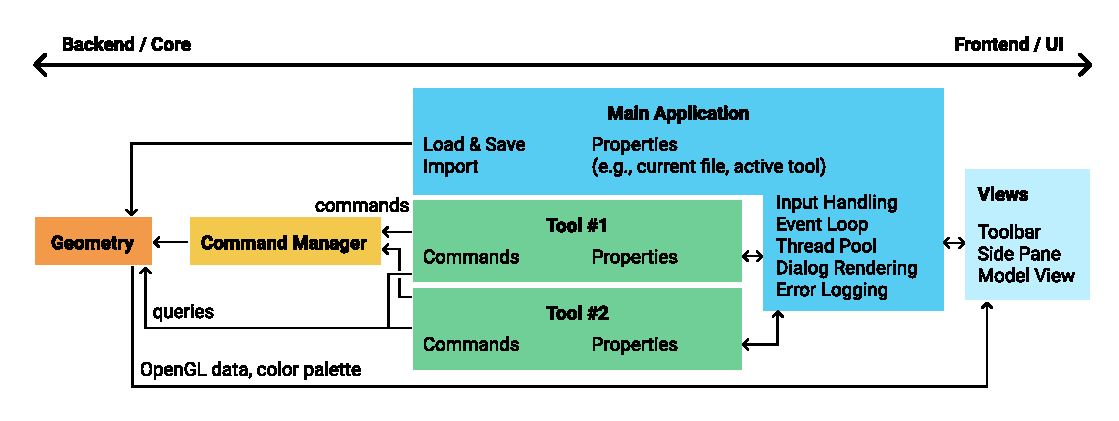
\includegraphics[scale=0.9]{images/diagram.eps}}
	\caption{An overview of the Pepr3D architecture.}
	\label{fig:architecture}
\end{figure}

\begin{itemize}
\item \textbf{Main Application} is the owner of the whole architecture. It contains functionality which is important for the whole application (like thread pooling or error logging) and owns and contains the other data structures. It acts as a single source of truth, holding the data that is valid at every moment (like the selected tool or the current model). This data is then fetched from the \texttt{MainApplication} by other components.

\item \textbf{Views} are the elements that fill the screen of the application. They handle rendering the user interface and allowing the user to perform basic actions to handle Pepr3D like rotating and zooming in on the model in \texttt{ModelView}, choosing a tool from the \texttt{Toolbar} or changing the tool's properties in \texttt{SidePane}.

\item \textbf{Tools} are the component that allows the user to interact with the data. Each tool has its properties that can be changed by the user via the user interface. If the user wishes to perform an action that would change the geometry (like colouring a triangle), the tool invokes a command which will take care of the action. The tool specifies how the right panel (\texttt{SidePane}) will look for each tool and can also query the \texttt{Geometry} class for simple information like the hovered triangle id.

\item \textbf{Command Manager and Commands} are the way Pepr3D handles the \textit{Undo} and \textit{Redo} operations. A \texttt{Command} is a single operation that can be ran by the \texttt{CommandManager} or joined with other \texttt{Command}s. A simple example of a command is the \texttt{PaintSingleColor} command. It takes a list of triangle ids and a color, and simply changes the color of those triangles to the new color. It can be joined with other \texttt{PaintSingleColor} commands, which have the same color by merging the two triangle id lists. The \texttt{CommandManager} then holds the stack of applied commands, saves the snapshots of the current geometry and is able to recreate any state by reverting to the older snapshots and running the commands again.

\item \textbf{Geometry} is the main data structure of the application. It holds the data of the triangles, their colors, normals, etc. It also generates the buffers for OpenGL and provides an API for the Commands (for non-\texttt{const} purposes) and Tools (for \texttt{const} purposes such as finding the hovered triangle id) to use.
\end{itemize}

The arrows between these components show the direction of communication between the components. We can see, for example, that only \texttt{CommandManager} and the \texttt{MainApplication} send data to \texttt{Geometry}, while the user interface does not know anything about the \texttt{CommandManager}. During the development we tried to separate the components as much as possible. Since our application is pretty basic, the pipeline is still connected quite a lot. We hope that this design is extendible though, and if the need arises, new components can be easily inserted into the overall architecture as illustrated in Figure \ref{fig:architecture}.

\section{Data flow}

In this section we demonstrate the data flow on a simple chain of operations an average user might perform. The sequence is the following and can be executed any time after launching the application: \textit{Import a model} $\rightarrow$ \textit{Select Bucket Painter tool} $\rightarrow$ \textit{Change settings on Bucket Painter} $\rightarrow$ \textit{Paint with the Bucket Painter} $\rightarrow$ \textit{Undo the operation}.

\begin{enumerate}
\item \textbf{Importing a model} causes the \texttt{MainApplication} to launch a asynchronous function that loads the new model, calculates the data for both the \texttt{MainApplication} and \texttt{Geometry} objects. This information includes the data structures for geometry operations or the calculations to re-orient the model correctly in the \texttt{ModelView}. After this step is done, \texttt{MainApplication} gets updated and holds the new \texttt{Geometry} object, which changes the geometry.

\item \textbf{Selecting the Bucket Painter} is, according to Figure \ref{fig:architecture}, a change of the \texttt{MainApplication}'s property. This is done via the \texttt{Toolbar} view. Upon selecting the new tool, when the next frame starts rendering, the \texttt{SidePane} will query the \texttt{MainApplication} object for the current tool, which will be the Bucket Painter. The \texttt{SidePane} will then let the Bucket Painter render its own settings within the \texttt{SidePane}.

\item \textbf{Changing Bucket Painter's settings} is changing the tool's properties. It is done within the \texttt{SidePane} view, which the Bucket Painter fills with relevant UI widgets (buttons, checkboxes, etc.). Changing these widgets will change the Bucket Painter's properties.

\item \textbf{Painting with Bucket Painter} by clicking on a certain triangle of the model. By clicking into the model view, an event gets created. The event is first processed in the \texttt{MainApplication} (e.g. if it is a \textit{drag and drop} event), then gets evaluated in \texttt{ModelView} (e.g. if it is a right click to rotate the view) and the \texttt{ModelView} then passes it into the tool, if it is required. The Bucket Painter gets the left click, queries the \texttt{Geometry} for the hovered triangle id, queries the \texttt{Geometry} again for the bucket spread and then executes a \texttt{PaintSingleColor} command. This command gets enqueued into the \texttt{CommandManager}, which executes it, changing the \texttt{Geometry}. In the next rendering frame, the \texttt{ModelView} notices, that the OpenGL geometry buffers are dirty, asks the \texttt{Geometry} to recalculate the buffers and renders the new colors.

\item \textbf{Undoing the last command} by clicking the \textit{Undo} button invokes the \texttt{CommandManager}. It restores the last snapshot of the \texttt{Geometry}, then re-runs all commands except the last one and updates the \texttt{Geometry}. This effectively restores the state before clicking with the Bucket Painter.
\end{enumerate}

This simple sequence of operations describes the majority of the program runtime data flow and control handling. It highlights important concepts of the UI -- such as the tool's user interface being rendered by the tool itself or the \texttt{CommandManager} semantics.

% In the following, elaborate on classes, what they do, how they are connected, what is ours/what is a library thing.
\chapter{Geometry}

In this chapter we describe the \texttt{Geometry} class in detail. We also discuss the other helper classes which handle geometry in Pepr3D.

\label{chap:geom}

\section{Geometry}

\subsection{Geometry}

\texttt{Geometry} is the main class of the whole data pipeline in Pepr3D. Here we explain the high-level details of this class, to hopefully give the reader a broader picture of the architecture, which makes navigating the code much easier. Since the class is rather large, we will not present a complete overview as in the following sections, but rather discuss several parts separately.

\subsubsection{Public data members}

The class itself does not provide any data as public. This is because it holds the geometry model, which cannot and should not be easily altered, since altering requires non-trivial re-computations (such as the acceleration tree structure or the Polyhedral surface data structure).

\subsubsection{Private data members}

All of the class' data is stored in private members, we present a list of the most important ones here:

\begin{lstlisting}
std::vector<DataTriangle> mTriangles;
std::map<size_t, TriangleDetail> mTriangleDetails;

std::unique_ptr<Tree> mTree;
std::unique_ptr<Tree> mTreeDetailed;

PolyhedronData mPolyhedronData;
std::unique_ptr<PolyhedronData::Mesh> mMeshDetailed;

std::unique_ptr<BoundingBox> mBoundingBox;
ColorManager mColorManager;

friend class cereal::access;
OpenGlData mOgl;
\end{lstlisting}

As we can see, the members are of two main functions: the ones holding the actual data (such as \texttt{mTriangles} and \texttt{mTriangleDetails}) and data structures built upon the data, which help us perform the operations quickly. There are several more conversion \texttt{std::map} objects which help the user retrieve the correct triangle data with an arbitrary information about the triangle (an id, a pointer in the surface mesh, etc.), which are not listed here for clarity's sake.

The \texttt{mTriangles} array functions as one would expect -- this is the main array, which stores the basic information for each triangle (the position, normals, etc.). If the \textit{Brush} or \textit{Text} tools are used, the triangles get split into detailed ones, and \texttt{mTriangleDetails} needs to be utilized to look up information about a triangle.

The \texttt{Tree} structure is CGAL's AABB hierarchical search tree which allows us to intersect the model with rays. This is especially useful during the user interaction (retrieving the triangle id which corresponds to the user-clicked triangle).

We also point out the duality of many of these data structures -- \texttt{mTree} and it's detailed version, as well as the  \texttt{PolyhedronData} object and it's detailed version. This is required, because the user can change the geometry of the model extensively by adding new details. Changing the geometry then alters the behaviour of several algorithms -- a \textit{breath-first} search behaves differently on a non-detailed model and a detailed model. However, completely discarding the non-detailed version is not wise either, since some operations may be faster to perform on the non-detailed versions, if the result does not depend on whether the mesh is detailed or not (for example, finding a position of ray-model intersection does not depend on any added details and should utilize the \texttt{mTree} member).

The last notable members are the \textbf{cereal} friend access and \textbf{OpenGL} buffer object. Cereal requires friend access to the class if we want the class to be exported. Since \texttt{Geometry} is the most important data object in Pepr3D, we obviously want to be able to save parts of it. The \texttt{OpenGlData} object is used to transport the geometry to the front-end rendering part of Pepr3D. The \texttt{Geometry} class creates and updates the buffers, and the front-end only re-renders the model when the buffers are changed. This way the front-end does not have to have any knowledge about the geometry and can be kept separate.

\subsubsection{Public methods}

The main way to work with the \texttt{Geometry} class. They can be divided into two obvious categories: the \textit{getters} and the rest.

We provide a lot of getter methods, so the user has a good way of communicating with the object and can extract as much information out as he wants. Most of the getter methods are \texttt{const}, since changing certain members is not allowed. There are, however, several which permit the user to change them, since the effect is immediate and doesn't have deeper consequences (like changing the colour palette in the \texttt{ColorManager}).

The other category of the methods are the algorithms used to implement Pepr3D's tools, load the data correctly and compute the necessary information. We list a few of the most important ones here:

\begin{lstlisting}
// Loading and computation
void computeSdfValues();
void loadNewGeometry(const std::string& fileName);
void recomputeFromData();
GeometryState saveState() const;
void loadState(const GeometryState&);

// Algorithms
std::optional<size_t> intersectMesh(const ci::Ray& ray) const;
template <typename StoppingCondition>
std::vector<size_t> bucket(const size_t startTriangle, const StoppingCondition& stopFunctor);
void paintAreaWithSphere(const ci::Ray& ray, const BrushSettings& settings);
void paintWithShape(const ci::Ray& ray, const std::vector<Point3>& shape, size_t color, bool paintBackfaces = false);
size_t segmentation( ... );
\end{lstlisting}

The first few methods are the main way to alter the \texttt{Geometry} and perform computations on the loaded model. The first batch of methods provides the tools to load and save the model correctly, as well as recompute the data if required (e.g. if a bug was encountered and the data is corrupted). Many of these methods utilize the \texttt{GeometryProgress} capability of Pepr3D, which allows the user to know how long the selected operation will run, or at least re-assures him that Pepr3D has not frozen.

The second group of methods are the algorithms employed to implement all the tools in the release version. We describe these methods in greater detail here:

\begin{itemize}
\item \texttt{intersectMesh(ray)} is the main method used to transform the user's clicks with tools into the geometry pipeline. Given a ray, this returns the id of the triangle which got intersected by the ray. Modern \texttt{std::optional} is utilized to avoid various "return codes" (like returning -1 for \textit{no hit}).

\item \texttt{bucket(startTriangle, stoppingCriterion} is used in several tools and implements the \textit{breath-first} search over a 3D triangle mesh. The \textit{BFS} traverses the mesh triangle to triangle until it is stopped by the stopping criterion. This criterion corresponds to the user interface of the \textit{Bucket} tool -- the user can either select to never stop, to stop upon meeting a different color, to stop on sharp edges or a combination of both. Modern C++ template approach is utilized to replace the runtime \texttt{if-else} decisions with compile time template processing.

\item \texttt{paintWith} are two methods used by the \textit{Brush} and \textit{Text} tools. They allow to paint with selected settings along a target ray. \texttt{paintAreaWithSphere} only paints a circular region on the surface of the mesh, where the circle is computed as the intersection of a sphere placed on the surface of the mesh with the mesh's sides. \texttt{paintWithShape} accepts a \texttt{shape} vector composed of points in 3D space and allows the user to paint a custom shape onto the mesh's surface.

\item \texttt{segmentation} implements the \textit{Automatic segmentation} tool by using the CGAL library, namely the \textit{Triangulated Surface Mesh Segmentation} \footnote{https://doc.cgal.org/latest/Surface\_mesh\_segmentation/index.html}. This process is dependant on the SDF values being calculated, which can be done with the computation method \texttt{computeSdfValues}.
\end{itemize}

\subsubsection{Private methods}

We will only describe a handful of private methods, since they are largely unimportant and only contain technical details which are not required for a general understanding. We will, however, mention the \textbf{OpenGL} buffer generators, since this is something not obvious from the first look on the \texttt{Geometry} class. As we have already mentioned above, the \texttt{Geometry} class handles all the buffer creation and keeps the buffers up-to-date, which allows us to shield the front end from the \texttt{Geometry} structure completely. If the structure of the geometry class changes, no further changes in the rendering front end code are required. The only thing which is required is to keep these methods correct. Namely:

\begin{lstlisting}
void generateVertexBuffer();
void generateIndexBuffer();
void generateColorBuffer();
void generateNormalBuffer();
void generateHighlightBuffer();
\end{lstlisting}

Further information is available in the \textit{doxygen} documentation or directly in the code.

\subsection{Triangle Detail}

\texttt{TriangleDetail}

\textbf{TODO after @ LUIS sends info}

\subsection{Detailed Triangle Id}

This \texttt{struct} is a very simple object, but important to understand, so we present it here, even though it is not a complex or confusing concept. It is a way to connect the original triangles with the detailed ones, once the user paints with the \textit{Brush} or uses the \textit{Text} tool. Before the user uses these tools, each triangle has its own id -- a \texttt{size\_t} type number. However, once the triangles are subdivided by use of one of these tools, this is no longer the case, since we are adding new triangles. The tools also support re-merging and simplifying the topology if the user removes the details by painting over them again. This would not be possible if we simply added the new triangles to the end and kept indexing by the \texttt{size\_t}, hence why we use this, admittedly more complex way of indexing.

\begin{lstlisting}
struct DetailedTriangleId {
    DetailedTriangleId()
    explicit DetailedTriangleId(size_t baseId, std::optional<size_t> detailId = {})

    size_t getBaseId() const;
    std::optional<size_t> getDetailId();

    bool operator==(const DetailedTriangleId& other) const;

   private:
    size_t mBaseId;
    std::optional<size_t> mDetailId;
};
\end{lstlisting}

The \texttt{BaseId} property is the triangle id of the original triangle, that has been split into many more. The \texttt{DetailId} is the id of the one of the smaller triangles, which form the original one (the one identified by \texttt{BaseId}).

A triangle which has not been subdivided, will have the \texttt{DetailId} empty, which indicates it is a base triangle. A triangle which formed by subdividing an already existing triangle, will have the \texttt{BaseId} equal to the id of the triangle which it has subdivided -- used to look up the \texttt{TriangleDetail} object in \texttt{mTriangleDetails}, and the \texttt{DetailId} will be used to look up the actual triangle, within this object.

\subsection{Data Triangle}

\texttt{DataTriangle} is the main way the geometry is stored in Pepr3D. It is a custom wrapper around \textit{CGAL}'s \texttt{Triangle\_3} class. Adding this wrapper allows us to attach additional information to each triangle. The information attached in our case is:

\begin{itemize}
\item \textbf{mColor} which is the color of the triangle. This is kept in a \texttt{size\_t} variable, because it refers to the index of the color in the color palette.

\item \textbf{mNormal} which is the normal vector of the triangle face. This is calculated as an average of the vertex normals of the triangle.

\end{itemize}

A second important class to talk about in this section is the \texttt{Data\-Triangle\-AABB\-Primitive}. This class provides the conversion between our \texttt{Data\-Triangle} (which contains a \texttt{CGAL::Triangle\_3}) and the \texttt{CGAL::AABB\_tree} which requires \texttt{CGAL::Triangle\_3} as input to build the tree around. We provide the tree our \texttt{Data\-Triangle} array and the tree converts it into \texttt{Data\-Triangle\-AABB\-Primitive}, which it accepts as a geometry primitive.

\section{Model Importer}

One of the classes included in this section is the \textit{Model Importer}. As the name suggests, this class handles the import of a new triangle mesh model into Pepr3D. This class heavily utilizes the \textit{Assimp} library we have mentioned several times in both the specification and documentation. Here is a quick overview of the class:

\begin{lstlisting}

class ModelImporter {
    std::string mPath;
    std::vector<DataTriangle> mTriangles;

    ColorManager mPalette;
    bool mModelLoaded = false;

    std::vector<glm::vec3> mVertexBuffer;
    std::vector<std::array<size_t, 3>> mIndexBuffer;

    GeometryProgress *mProgress;

   public:
    ModelImporter(const std::string p, GeometryProgress *progress, ::ThreadPool &threadPool);
    bool isModelLoaded();

    ColorManager getColorManager() const;
    std::vector<DataTriangle> getTriangles() const;
    std::vector<glm::vec3> getVertexBuffer() const;
    std::vector<std::array<size_t, 3>> getIndexBuffer() const;
}

\end{lstlisting}

We will now go through the public API of the class, explaining in detail what each method does and why it is needed.

Firstly, \texttt{ModelImporter} gets initialized using its constructor. It gets the path to the file and our persistent threadpool, as well as a \texttt{GeometryProgress} object, which is used to report the import progress to the UI. This setup makes a single ModelImporter object responsible for a single imported mesh file, which follows the \textit{Resource Acquisition Is Initialization} or \textit{RAII} \footnote{https://en.cppreference.com/w/cpp/language/raii} principle, which is prevalent in the C++ scene. Once initialized, the \texttt{ModelImporter} can now return all the data it loaded.

A simple check of \texttt{ModelImporter}'s ready status can be performed using the method \texttt{isModelLoaded()}. This should primarily be used in combination with C++'s \texttt{assert} call.

Once the model is loaded correctly, the object now provides the data it has loaded. There are several methods to retrieve data.

\begin{itemize}
\item \texttt{getColorManager()} is a method which returns a \texttt{ColorManager} object, initialized with the colors of the imported file. This means that if a coloured geometry file gets loaded, the \texttt{ModelImporter} will automatically create a coloured model which is then displayed in Pepr3D. It will also initialize the color palette with the model's colors, not with the default ones.

\item \texttt{getTriangles()} is the most important method of the class. This method returns an array of \texttt{DataTriangle} objects. This is the main data Pepr3D works on. These returned triangles are preprocessed using both \textit{Assimp} preprocessing options and our own. Examples of preprocessing include triangulating all non-triangle primitives (like quads), removing duplicated vertices and removing degenerate triangles (with a zero area).

\item The pair of methods \texttt{getVertexBuffer()} and \texttt{getIndexBuffer()} is a secondary means of extracting the same geometry data as in the \texttt{getTriangles} method, but this time in the "OpenGL" format of a vertex buffer and an index buffer. This data is used only during the construction of the polyhedron model for the \textit{CGAL} library. Extracting the secondary data is easier and faster than transforming the \texttt{DataTriangle} array back into this buffer representation just for the polyhedron build.

\end{itemize}

Most of the private members are very self-explanatory, we will, however, briefly comment on the \texttt{mProgress} object. This object takes advantage of \textit{Assimp}'s ability to report the percentage-wise progress during loading and preprocessing. We use this information in the loading dialog, to notify the user on the progress of the import. This makes it clear to the that the program is working as intended and has not crashed or stopped.

\section{Model Exporter}

The \texttt{ModelExporter} is an easy to use class which handles the export of the model. Once again, it is initialized once for every geometry object (a model) and can get called multiple times if we are saving the same geometry data (maybe with different parameters) multiple times. Once a new model gets loaded, a new \texttt{ModelExporter} needs to be initialized. Here is a simple overview of the class:

\begin{lstlisting}
class ModelExporter {
    const Geometry *mGeometry;

    GeometryProgress *mProgress;
    std::vector<float> mExtrusioCoef;

   public:
    ModelExporter(const Geometry *geometry, GeometryProgress *progress);

    void setExtrusionCoef(std::vector<float> extrusionCoef);

    bool saveModel(const std::string filePath, const std::string fileName, const std::string fileType, ExportType exportType);

    std::map<colorIndex, std::unique_ptr<aiScene>> createScenes(ExportType exportType);
}

\end{lstlisting}

There are a few basic methods which we will cover first, as well as an extra degree of freedom for the users of this class, which requires a bit more knowledge, which we explain at the end.

\begin{itemize}

\item The \textit{constructor} takes a pointer to the current \texttt{Geometry} object and a pointer to a progress indicator. Here we again exploit \textit{Assimp's} progress reporting functionality to let the user know how far along the export is.

\item \texttt{setExtrusionCoef()} is a simple \textit{setter} which allows the user to specify the depth of extrusion for each segment.

\item \texttt{saveModel()} is the main method the users will call if they wish to proceed with the export in the current setup. The user specifies the file path, file name and file type of the export, as well as which export should get used, as there are several options.
\end{itemize}

We mentioned several options of exporting, which are decided by the \texttt{ExportType} enumerator. The whole definition of this \texttt{enum} is:

\begin{lstlisting}
enum class ExportType { Surface, NonPolySurface, NonPolyExtrusion, PolyExtrusion, PolyExtrusionWithSDF };
\end{lstlisting}

The only options the end user has are exporting only in \texttt{Surface} mode or in \texttt{Extrusion} mode, with the ability to turn on \textit{SDF limitation} when in the \texttt{Extrusion} mode. The two options prefaced with the keyword \texttt{Poly} are there for the developers, since these get invoked when the loaded model cannot be built into a polyhedron structure (which is displayed as a warning dialog, which is covered in greater detail in Chapter \ref{ch:ui}.

The last public method of the class is \texttt{createScenes()}. This is an advanced method which gives the developer access to the segmented scenes. This can be used, for example, to allow the user to preview the export results directly in Pepr3D (as it is done in the \textit{Export Assistant}).

\section{Font processing}
\label{sec:fonts}

Big portion of the code of this class is based on the \textit{Font23D} library which can be found on GitHub \footnote{https://github.com/codetiger/Font23D}. The team read through the code, heavily modified it to transform it from the \textit{C} language to the modern \textit{C++} and built a new class around what were only free methods in \textit{Font23D}. This object also uses the \textit{FreeType}, \textit{FTGL} and \textit{Poly2Tri} libraries.

The main goal of the \texttt{FontRasterizer} class is to take smooth bezier curves of letters from the \texttt{.ttf} font files and transform them into a triangle mesh, with a variable rasterization steps. These meshes are then used in the \textbf{Text} tool.

A simple overview of the \texttt{FontRasterizer} class follows:

\begin{lstlisting}
class FontRasterizer {
   private:
	struct Tri {
        glm::vec3 a, b, c;
    };

    std::string mFontFile;
    bool mFontLoaded = false;

    FT_Library mLibrary;
    FT_Face mFace;
    FT_UInt mPrevCharIndex = 0, mCurCharIndex = 0;
    FT_Pos mPrev_rsb_delta = 0;

   public:
    FontRasterizer(const std::string fontFile);
    std::string getCurrentFont() const;
    bool isValid() const;

    std::vector<std::vector<FontRasterizer::Tri>> rasterizeText(const std::string textString, const size_t fontHeight, const size_t bezierSteps);
}
\end{lstlisting}

As we can see, similar to the \texttt{ModelImporter} class, this class also uses the \textit{RAII} principle, this time to load and hold the font face, loaded from a \texttt{.ttf} file. Once the font file is loaded successfully, the object can then convert any text into a triangle mesh.

The interface of this class is rather simple -- the constructor takes a single \texttt{std::string}, which is the path to the font file. The API provides a \texttt{isValid()} method to check whether the initialization was performed correctly. The API also provides the font file name, without the whole path, which can be accessed by the method \texttt{getCurrentFont()}. This is used in the user interface to display the currently selected font.

The main method of the class is the \texttt{rasterizeText()}. It takes a \texttt{std::string} containing the text the user wants to convert to triangles, the \texttt{fontHeight} integer, which corresponds to the font height commonly found in text editors and the variable \texttt{bezierSteps}, which allows the user to control the roughness of the approximation. The useful range of the \texttt{bezierSteps} variable is around $1$ -- $5$. $1$ yields very rough results, useful for "blocky" fonts like \textit{Impact}, while $3$ should be sufficient for any standard font. For high precision, a higher setting should be used. Please note that the higher the \texttt{bezierSteps}, the more triangles will be generated.

Last thing to note, is the custom triangle object the \texttt{rasterizeText} method returns. \texttt{Tri} is a custom \texttt{struct} declared private in \texttt{FontRasterizer}. This is done to achieve two things: 

\begin{enumerate}
\item \texttt{FontRasterizer::Tri} should not be used outside of the class. It is a temporary type and is useful only to the \texttt{FontRasterizer} class. The private definition prevents this behaviour. Users should not create more objects of this type at any time.

\item \texttt{FontRasterizer::Tri} is returned by \texttt{rasterizeText}. This is because we want the \texttt{FontRasterizer} to be an independent class, which can be used on its own and not depend on any Pepr3D types. Returning a custom type achieves this behaviour, and it is expected that the users will want to convert the outcome into a custom type more often than not anyway.
\end{enumerate}

\section{Color Manager}

The \texttt{ColorManager} is a simple class which manages the current color palette. At most one \texttt{ColorManager} is active, which is the one \texttt{MainApplication} holds as a source of truth. \texttt{ModelImporter} also creates a new \texttt{ColorManager} while importing an already-coloured model.

Now we list a simplified overview of the class:

\begin{lstlisting}
class ColorManager {
   public:
    using ColorMap = std::vector<glm::vec4>;

   private:
    ColorMap mColorMap;
    size_t mActiveColorIndex = 0;

    friend class cereal::access;

   public:
    ColorManager();
    ColorManager(const ColorMap::const_iterator start, const ColorMap::const_iterator end);
    explicit ColorManager(const size_t number);

    void addColor(const glm::vec4 newColor);
    void setColor(const size_t i, const glm::vec4 newColor);
    void replaceColors(const ColorMap::const_iterator start, const ColorMap::const_iterator end);
    void replaceColors(const ColorMap& newColors);
    glm::vec4 getColor(const size_t i) const;

    size_t getActiveColorIndex() const;
    void setActiveColorIndex(size_t index);

    static void generateColors(const size_t colorCount, std::vector<glm::vec4>& outNewColors);
}
\end{lstlisting}

As we can see, \texttt{ColorManager} is basically a simple wrapper around STL's \texttt{std::vector}, specialized on holding \texttt{glm::vec4} and extended with some color-generation features. It also is responsible for handling the current active color in the \texttt{mActiveColorIndex} member variable. This is the color the user has currently selected in his color palette widget.

There are several ways to initialize the \texttt{ColorManager}. You can initialize it to the default palette, with a list of colors or simply with a number of colors you require. In the last case, the \texttt{ColorManager} will generate new colors, which will be \textit{visibly distinct} from each other (you will not get 3 slightly different shades of blue). The generation is done using the \texttt{generateColors()} method.

The \texttt{ColorManager} API has all the different calls you could expect from a \texttt{std::vector} wrapper, like \texttt{empty()}, \texttt{size()} and \texttt{clear()}, which we have omitted from the overview for clarity.

The most important part of the API are the \texttt{addColor()}, \texttt{setColor()} and \texttt{replaceColors()} methods. These allow for changing of the palette on the fly. Note that changing the palette changes the colors on the model in real time. \texttt{getColor()} can be used to query the \texttt{ColorManager} on any color (for example for user interface purposes), and when combined with the following pair of methods, it provides a vital part of Pepr3D by allowing the color palette widget to work.

We have already mentioned one of the two remaining methods -- the getter \texttt{getActiveColorIndex()} and the setter \texttt{setActiveColorIndex()}. These methods are invoked when the user changes the active color in the color palette widget in the user interface. They are also invoked by various tools when the tool is constructing the recolour command and needs to know which colour the user painted with.
\chapter{Commands and Command Manager}

In this chapter, we discuss the command system that provides the \textit{Undo} and \textit{Redo} capability of Pepr3D. First we explain the \texttt{Command} class in detail and then we show how the \texttt{CommandManager} operates to provide a fully functioning \textit{Undo} and \textit{Redo}.

\section{Commands}

Commands are the primary means of altering the geometry model. Each of them gets executed and placed on the command stack, which allows for the Undo and Redo operations to function correctly. The commands then interact with the geometry model to modify it according to the user's wishes.

Because each command gets put on the command stack, and each Undo step removes one command from the stack, each command has to have a visual impact on the user's work. This means that internal computations, such as geometry queries, cannot be represented as commands, because pressing the Undo button would not have any visual effect and would confuse the user. Examples of commands include: colouring a single triangle (triangle painter tool), colouring multiple triangles (like in bucket painter) or changing the color palette.

A single command is a class derived from the \texttt{CommandBase} class, which has this structure:

\begin{lstlisting}
template <typename Target>
class CommandBase {
    template <typename>
    friend class CommandManager;
   public:

    CommandBase(bool isSlow = false, bool canBeJoined = false);

    virtual std::string_view getDescription() const = 0;
    bool isSlowCommand() const;
    bool canBeJoined() const;

   protected:
    virtual void run(Target& target) const = 0;
    virtual bool joinCommand(const CommandBase&)

   private:
    const bool mIsSlow;
    const bool mCanBeJoined;
};
\end{lstlisting}

As we can see, there are only a few methods to implement per each command. Namely \texttt{run()} and \texttt{joinCommand()}. The only properties of the command are \texttt{mIsSlow} and \texttt{mCanBeJoined}, which are (through their const getters) accessed by the \texttt{CommandManager}.

The \texttt{mIsSlow} property notifies the \texttt{CommandManager} about a slow command, which means a snapshot should be made to allow for quicker undoing and redoing (we will refer to both of these options as only "undo" from now on).

The \texttt{mCanBeJoined} property allows the \texttt{CommandManager} to join two commands of the same type together.

Now that we know how commands look like and work, we can look at the \texttt{CommandManager} class and see how the entire feature is implemented in Pepr3D.

\section{Command Manager}

The centrepiece of the \texttt{CommandManager} is the \textbf{command stack}. The Command Stack is a \textit{LIFO} type structure, with the main purpose to store the executed commands, which allows the \texttt{CommandManager} to perform the undo operations. This data structure is then operated by the \texttt{CommandManager}. Following is the overview of the \texttt{CommandManager} class.

\begin{lstlisting}
template <typename Target>
class CommandManager {
   public:
    using CommandBaseType = CommandBase<Target>;
    using StateType = decltype(std::declval<const Target>().saveState());
    static const int SNAPSHOT_FREQUENCY = 10;

    explicit CommandManager(Target& target);

    void execute(std::unique_ptr<CommandBaseType>&& command, bool join = false);

    void undo();
    void redo();

    bool canUndo() const;
    bool canRedo() const;
    const CommandBaseType& getLastCommand() const;
    const CommandBaseType& getNextCommand() const;
    size_t getVersionNumber() const;

   private:
    Target& mTarget;
    std::vector<std::unique_ptr<CommandBaseType>> mCommandHistory;
    size_t mPosFromEnd = 0;
    size_t mVersion = 0;

    struct SnapshotPair {
        StateType state;
        size_t nextCommandIdx;
    };
    std::vector<SnapshotPair> mTargetSnapshots;
};
\end{lstlisting}

As we can see, the class is not complex. It operates over a templated class \texttt{Target}, which only has to be able to be able to load its state and save its state using the methods \texttt{loadState} and \texttt{saveState}. The state is what gets undone during the undo operation.

The three main methods to operate the undo pipeline are \texttt{execute()}, \texttt{undo()} and \texttt{redo()}, which are self-explanatory. The user interface can also use the methods \texttt{canUndo()} and \texttt{canRedo()} to notify the user with visual cues (like emboldening the undo signs) if the undo and redo actions are available.

The \texttt{CommandManager} also keeps its current cumulative version, which gets incremented during each \texttt{execute()}, \texttt{undo()} and \texttt{redo()}. This is a way to keep track of the user's actions and notify him if the current project was modified after it was saved.

The main data is stored in the \textit{command stack}, which have already discussed. The command stack is the member \texttt{mCommandHistory}, which holds all past commands in a \texttt{std::vector}, which is a sufficient structure to implement a \textit{LIFO} in. It holds pointers to the commands, instead of commands themselves to be able to use \textbf{polymorphism} in C++. The pointers are realised with C++'s \texttt{unique\_ptr} for maximum memory safety.

After consideration, we chose the snapshotting technique we discussed in the \textit{Specification document}. Snapshotting happens inside the \texttt{execute()} method and is regulated by one member variable inside the \texttt{CommandManager} -- the \texttt{SNAPSHOT\_FREQUENCY}. \texttt{mTargetSnapshots} is the array which holds the already taken snapshots. This \texttt{std::vector} gets manipulated during \texttt{execute()} and \texttt{redo()} to correctly perform the undo and redo functions. Snapshots are saved as a \texttt{SnapshotPair}, which remembers the current state and the command id which it was taken at.

Let's now illustrate the redo realised by snapshotting on a specific example. Let there be $C$ commands on the command stack, with last snapshot taken at the $S$-th command, where $S < C - 1$. If we now undo, which means point the current Target state at $C - 1$, the last \texttt{SnapshotPair} gets inspected, and we find that the command id of the last snapshot was $S$. The state gets re-instantiated to the state we found in the \texttt{SnapshotPair}. Now we need to re-apply all commands from $S+1$ to $C-1$ to be correctly back in the $C-1$ state.
\chapter{Core modules}

This chapter takes a closer look at the portion of the architecture highlighted in Figure \ref{fig:architecture_commandstack}. We will explain how each task is performed once the UI element has received the input from the user. The UI portion of the architecture will be covered in the next chapter.

\begin{figure}[h]
	\centering
	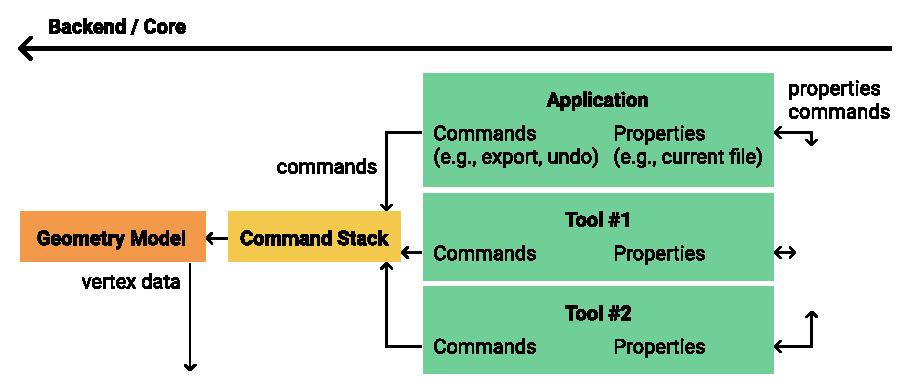
\includegraphics[scale=0.9]{images/architecture_core}
	\caption{The part of architecture covered in this chapter.}
	\label{fig:architecture_commandstack}
\end{figure}

% TODO: WARNING: CAREFUL, JE UI NEXT NEBO PREVIOUS CHAPTER?

\section{Commands}
Commands are the primary means of altering the geometry model. Each of them gets executed and placed on the command stack, which allows for the \textit{Undo and Redo} operations to function correctly. The commands then interact with the geometry model (this interaction will be explained in greater detail in section \ref{geometrymodel}) to modify it according to the user's wishes.

Because each command gets put on the command stack, and each Undo step removes one command from the stack, each command has to have a visual impact on the user's work. This means that internal computations, such as geometry queries, cannot be represented as commands, because pressing the Undo button would not have any visual effect and would confuse the user. Examples of commands include: coloring a single triangle (triangle painter tool), adding a brush stroke (as in semi-automatic segmentation we looked at in Chapter 2) or a single step of triangle mesh subdivision.

\subsection*{Implementation details}

There are several ways of implementing a command stack for \textit{Undo and Redo} operations, here we highlight two, each with its pros and cons. We expect to test both variants and see which works better. We will use $A$ to refer to the object \textbf{after} applying the newest command, and $B$ as the object \textbf{before} the latest command was applied.

One variant of the implementation requires each command to be able to perform the \textit{Undo} step by itself. This is usually done by remembering the state the object was before applying the command ($B$), and if \textit{Undo} is pressed, replacing the current object $A$ with the saved $B$. A command in this variant is a class with three primary methods.
\begin{itemize}
\item \textit{constructor} -- Once the command gets created, the main thing to do is remember the state the geometry model was in before the command modified it -- $B$. This will allow for the command to restore the model if \textit{Undo} is pressed. The advantage of saving the state in the constructor and not in the execute function itself is because of the \textit{Redo} mechanism -- if the user repeatedly presses the combination of \textit{Undo + Redo}, the model gets saved only once as opposed to each execute.
\item \textit{execute()} -- The execute function will perform the task the command is created to do. This will typically get called immediately before the command gets placed onto the command stack. This will change the object $B$ into the object $A$.
\item \textit{undo()} -- This method will take the state of the model saved by the constructor of the command and apply it to the current geometry model $A$, effectively reversing the command and obtaining $B$. In other words, this method will change the object $A$ into the object $B$.
\end{itemize}

This variant is mostly desirable if the operations can be undone easily (e.g. deleting a single letter is a very easy operation to undo). For our purpose, this approach might not be the best because geometric operations usually do not have an easy inverse operation. This means that each command would have to save the whole state of the geometric model, which might prove too straining on the computer's memory.

The other possible variant of implementation is snapshotting the model every few commands (with the latest snapshot called $S$), and when the user requests an undo, simply restoring the previous snapshot $S$, and re-applying every but the last command $L$. This version is a bit more CPU-intensive but should result in much less memory being used.

In this version of the implementation, the only method of the command class that remains from the previous list is \textbf{execute()}, as all others are managed by the command manager.

\section{Command Manager and Command Stack}

\subsection{Command Stack}

As the name suggests, the Command Stack is a \textit{LIFO} type structure, its main purpose to store the executed commands to allow for the \textit{Undo and Redo} operations to be performed. As we have outlined in the previous section, either each command carries all necessary information to perform both actions (in the first variant) or the command manager remembers the snapshots and is able to perform the \textit{Undo and Redo} actions. Hence the Command Stack can only be a simple container without any significant logic behind it.

\subsection{Command Manager}

The command manager is a object to manage the command stack. It receives the commands from tools, executes them and stores them in the command stack.

In the first variant of the implementation, when the user wishes to \textit{Undo} an operation, the command manager retrieves the top command from the stack ($L$) and invokes its undo() method, replacing the current $A$ with the original $B$.

In the second variant of the implementation, the command manager also saves the complete geometric data every $N$ steps (we expect $N < 5$) -- so called \textit{snapshots}. The snapshotting is invoked during after the \textit{execute()} method of the incoming command gets called. When the user wishes to \textit{Undo} an operation, the command manager retrieves the last snapshot $S$, $i$ commands behind the current model. It then re-applies all commands from $i+1$ to the next to last command (ending before applying $L$), effectively \textit{undoing} the operation and replacing the current $A$ with the original $B$. Unlike the previous version, the state $B$ is not saved anywhere but it is re-constructed from the last $i-1$ commands that originally transformed $S$ into $B$.

\section{Tools}

A tool is the main programable component which connects the low-level command structure we outlined above and the high-level UI components (such as color-pickers, the user performing brush strokes and file operations like exporting the file). This design should also allow for later advancements of the software easily -- adding a tool to the software should be a matter of writing the new tool's Tool class, unless the tool is advanced and needs some complicated custom geometry processing functions.

\medskip

Each tool is composed of two main components:
\begin{itemize}
\item \textit{properties} -- a methodless object holding the tool's properties which can be customized by the user. This includes, for example, the color which gets assigned to the triangles in the triangle painter tool, the number of colors for automatic-segmentation, the subdivision level or the gradient thresholds for region detection in bucket painting. The information in this object gets changed directly when the user interacts with the UI.

\item \textit{commands} -- Each tool generates at least one command, which it creates, fills with all necessary information the command needs to execute itself, and passes it to the command manager. More complicated tools can create more commands, as we will illustrate in the following section. The tool is able to do some pre-processing before a command is issued, in case the pre-processing isn't visible on the screen, as shown in example 4.1.

\end{itemize}

\section{Examples of data flow within the center section of the achitecture}

We include a few example use cases which should illustrate what happens in the application (normal font) when a user interacts with the UI (italics). The first example shows the need for preprocessing power within the tool class, while the second example illustrates the need for multi-command tools.

\subsection{A preprocessing example - triangle painter}
\textit{The user selects the triangle painter from the tool box, and in the Side Pane, he changes the color from default red to green.}

This action makes the UI manager change the color property of the TrianglePainter tool from red to green.

\textit{The user then clicks on a triangle that he sees on the screen, in Model View.}

This makes the UI generate a ray in a direction of the user's mouse input. It then calls the TrianglePainter tool, passes the ray and tells it to color it, according to the tool's settings. The tool first calls the Geometry Model, to retrieve the triangle that gets intersected by the given ray, then creates a command to color the triangle with the color it has in its properties. The command is then passed to the CommandManager and executed. The query for the ray intersection is not passed as a command, because it is not visible for the user, hence should not be reversible.

\subsection{A multicommand tool example - the semi-automatic segmentation tool}
\textit{The user selects the number of colors -- 4. The user also selects which colors he would like to use -- C, M, Y, K.}

The UI updates the tool's properties to reflect these values.

\textit{The user then selects the color C, and performs a stroke.}

The UI first tells the tool that the current color is C. Then the tool receives the parameters of the stroke (much like the ray for a click), creates the command for a stroke with color C and sends it to the command manager.

This gets repeated for the other 3 colors. So far the tool generated 4 commands. If at any point the user presses Ctrl + Z, only one of the strokes disappears.

\textit{The user confirms the hint strokes are complete and the segmentation can start.}

The tool now generates the final command to complete the segmentation and passes it to the manager.


If the user presses Ctrl + Z now, only the segmentation will get removed, with the strokes still remaining on the object.

\section{Geometry model} \label{geometrymodel}

The geometry model is responsible for keeping the geometry data (triangles of the model) in memory and implementing geometric operations, that then get used in commands, to perform the tasks specified by the tools.

\subsection{Implementation variants}

There are two main approaches to programming the geometry model. One approach is to look at the model as a state-less chunk of data. The functions that operate on the model (e.g. \textit{return the triangle that intersects this ray}) are free functions that just get called on the geometry model. The second approach is to implement the model as a full object. This means that the model has its private data -- the triangles of the user's model, and it has its methods -- the geometric operations it allows the user (i.e. the programmer of the commands and tools) to perform upon the private data.

Both solutions have their pros and cons and we, at the time of writing, do not know which will shape up to be a better fit to the application. We will briefly mention some of the reasons we might choose either one. The state-less \textit{struct} version is better for handling the data. We will need to make some kinds of copies both for saving the model on the disc and for the \textit{undo Undo and Redo} operations. This approach would allow us to simply copy the struct and not waste any space or time. The object-oriented approach is easier to work with and probably less confusing for new programmers trying to implement a new tool or other extensions to the application.

\subsection{Libraries}

There are several libraries that the geometry model could benefit from. We have been searching on the internet and did research and we found the following libraries that we will try to use to augment the geometry model.

\begin{itemize}
\item \textbf{Assimp\footnote{http://www.assimp.org/}} -- a portable Open Source library to import various well-known 3D model formats in a uniform manner\footnote{Description taken from http://www.assimp.org/}. This library is very important to our application as it will allow us to support a plethora of 3D formats for the users to use. This should help the less experienced users by not forcing them to convert their objects to different formats before our program can import them.

\item \textbf{cereal\footnote{https://uscilab.github.io/cereal/}} -- cereal is a header-only C++11 serialization library. cereal takes arbitrary data types and reversibly turns them into different representations, such as compact binary encodings\footnote{Description taken from https://uscilab.github.io/cereal/}. We need to serialize data to enable saving the current state of the user's project on disc, and then be able to de-serialize them when the user wishes to continue working on the saved project and presses \textit{load existing project}. We have had positive experience with cereal and that is the reason we chose this library.

\item \textbf{The Computational Geometry Algorithms Library or CGAL\footnote{https://www.cgal.org/}} -- a software project that provides easy access to efficient and reliable geometric algorithms in the form of a C++ library\footnote{Description taken from https://www.cgal.org/}. We have heard very positive feedback on CGAL and therefore will attempt to use the library for the more complex geometry problems. We have, however, not had any previous experiences with CGAL, so we are unsure as to how well it will fulfill our requirements and might drop the use of it if it does not meet our expectations.
\end{itemize}
\chapter{User interface}

A \emph{user interface} (UI) is the front-facing part of Pepr3D that the users interact with.
It is responsible for managing windows, showing buttons, rendering the 3D model, handling mouse clicks, hotkeys, showing error dialogs, and much more.
In case of Pepr3D, it should be an easy-to-use, intuitive, and fast abstraction of the complex 3D geometric algorithms at the backend, see Figure~\ref{fig:diagram_ui}.

\medskip

We divide the Pepr3D UI into the following main parts:
%
\begin{itemize}
\setlength\itemsep{0em}
\item the \textbf{main application} corresponds to the whole main window, which consists of the following:
\item a \textbf{toolbar} with toggleable buttons representing tools, undo/redo, etc.,
\item a \textbf{side pane} with buttons, checkboxes, sliders, etc., representing configuration of the currently selected tool,
\item and a \textbf{model view} with the 3D model which the user can rotate, zoom, paint on it, etc.
\end{itemize}

\begin{figure}[h]
	\centering
	\centerline{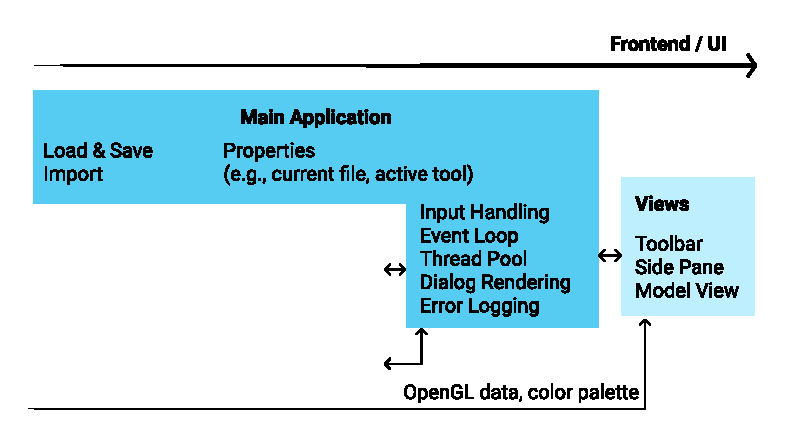
\includegraphics[scale=1.0]{images/diagram_ui.eps}}
	\caption{An overview of the Pepr3D UI architecture, based on Figure~\ref{fig:architecture}.}
	\label{fig:diagram_ui}
\end{figure}
\vspace{-1.5em}

\section{Key concepts}

In the specification of Pepr3D, we explained several main ideas that the user interface of Pepr3D is built around.
We will not repeat every single idea from the specification here as that would be redundant, but we explain the key concepts that we kept in mind while developing the user interface.

To prevent reinventing the wheel, our concepts are based on investigating how other developers implement user interfaces.
Our UI mainly consists of \emph{real-time 3D rendering}, i.e., displaying the 3D model that users can interact with, and \emph{widgets}, i.e., the windows, buttons, check boxes, text labels, etc.

\subsection{Real-time 3D rendering}

In Pepr3D, a regular user interface with a few buttons and texts is not enough.
We primarily need real-time 3D rendering and manipulation of the 3D model that the user is editing.
Hence the whole user interface needs to take this into account and is primarily based on real-time rendering.

As explained in our specification, when we were looking for a 3D rendering library, we mainly focused on finding an easy-to-use abstraction, e.g., for rendering 3D primitives, using custom shaders with uniforms, uploading textures to the GPU, keeping constant framerate, etc.
We decided to use \emph{Cinder}, which is also cross-platform and supports asynchronous events.

\subsection{Widgets}

\label{subsec:imgui}

As Pepr3D is based on real-time rendering, we decided to use \emph{immediate UI}, i.e., a procedural UI redrawn every frame that is mostly stateless.
This means that we do not have to program any explicit synchronization between the UI and the backend.
Whenever we re-render the UI, it will be rendered with the newest data.
Retained state is only where necessary, e.g., for complex calculations not needed in every frame.
Our immediate UI is a part of the 3D renderer based on Cinder and OpenGL, where the widgets are rendered on top of the scene.

We also kept in mind that \emph{presentation should be separated from the logic}, i.e., the rest of the application should know nothing about the UI at all.
Hence our UI depends on the backend, but the backend does not depend on the UI at all.
In theory, we are able to easily replace the UI with another, should it be necessary.

For these reasons and others explained in our specification, we based our widgets on a library called \emph{Dear ImGui}.
It provided us with basic handling of mouse clicks, keyboard inputs, etc., and also with 2D drawing such as texts, icons, buttons, etc.
But the design of Pepr3D is completely ours and is based on heavily customized widgets based on ImGui primitives.

\section{Application}

\label{sec:app}

The whole application and its main window are executed via the Cinder library.
The main file \texttt{main.cpp} contains a Cinder macro which corresponds to cross-platform \texttt{main} functions.
Cinder is responsible for creating an instance of our \texttt{MainApplication} class on which it calls the \texttt{setup} method.

After the main window is set up, Cinder keeps calling the \texttt{update} and \texttt{draw} methods every frame in this order.
Cinder also handles all necessary events from an operating system and calls the appropriate methods of the \texttt{MainApplication}.

\subsection{Main application}

The \texttt{MainApplication} class is a router which interacts with other components, mainly the three major UI components: a \textbf{toolbar}, a \textbf{side pane}, and a \textbf{model view}.
It instantiates them, listens for events from the operating system, and passes them to the components so that they can handle them themselves.

This also includes delegating hotkeys, open, save, import, and export commands to their dedicated classes, handling minimized application, etc.
We can say that every user interaction gets first through the \texttt{MainApplication} which then delegates it to other components.

Because of the Cinder API, setup is not done directly in the constructor, which only instantiates other components, but in the \texttt{setup} method which Cinder calls once it is ready.
It creates and configures debug and error loggers, sets the main window properties such as its resolution and icon, initializes ImGui, hotkeys, the default geometry (cube), and constructs all tools.

The \texttt{draw} method draws the major UI components and also renders existing modal dialogs and a progress indicator when necessary.
The \texttt{update} method checks invariants such as that the selected tool is not disabled, application is not rendered if minimized, and unsaved changes in a project are marked with an asterisk * in the title.

\subsection{Multi-threading and background tasks}

Some operations such as importing or exporting a large model may take a long time.
If everything was done in the main thread, rendering of the UI would be paused and the window would become unresponsive.
In UI applications, we want to avoid this by running slow operations in the background.

For this purpose, we use a very simple thread-pool library consisting of just a single \texttt{ThreadPool} class.
A single instance of this thread pool is stored as a static member of the \texttt{MainApplication}.

Delegating a task into the thread pool is done by calling \texttt{enqueue} on the thread pool.
This method returns a C++ \texttt{future} which we can wait for.
However, the UI in the main thread should \emph{not} wait for the tasks to finish in a blocking way, as that would defeat the purpose.

Instead, we can call \texttt{dispatchAsync} on the \texttt{MainApplication}, which dispatches another callback via Cinder.
This callback will be executed before a new frame starts rendering.
This enables the background tasks to notify the UI that they have finished.

In summary, the pipeline works like this: the UI enqueues a slow function $F$ (typically a lambda function) to the thread pool and continues rendering.
Right before $F$ finishes, the $F$ itself calls \texttt{dispatchAsync} with another function $A$, which will be run on the UI thread at a new frame.
$A$ is used to update the UI to the new state, e.g., after loading a new model.

\subsection{Resources of a minimized or obscured window}

Because Pepr3D runs at a vertically synchronized framerate (typically 60 frames per second), it uses CPU and GPU resources even when minimized or obscured.
We had to implement a way to pause rendering while the window is not visible.
Cinder provided a way to tell if the window was minimized, but it did not solve situations where a window was obscured but not technically minimized.

This proved to be a difficult problem that we managed to partially solve for Microsoft Windows by using the Windows API.
In regular intervals, we check whether the top left corner, center, and bottom right corner are obscured by another window of another application.
When they are, we pause the rendering.
This significantly lowers the CPU and GPU usage when Pepr3D is not used.

\subsection{Dialogs and fatal error handling}

In Pepr3D, there are 3 types of dialogs: general modal dialogs, a special export dialog, and a progress indicator.
All these dialogs are drawn from the \texttt{MainApplication} on top of everything else and all mouse and keyboard input for the rest of the components is paused.

\paragraph{General modal dialogs and fatal errors}
General modal dialogs are represented by the \texttt{Dialog} class and they can be of various importance, e.g., information dialogs, fatal error dialogs, etc.
The dialogs are stored in a priority queue with the most important dialog on top.
They can be pushed to the queue by calling \texttt{pushDialog} on the \texttt{MainApplication} instance.

When we detect an invalid state of the application, e.g., by catching a fatal exception, a \emph{fatal error dialog} is pushed to the queue.
When a fatal error dialog is on the top of the queue, rendering of all components is stopped and only the dialog is shown, because it cannot be guaranteed that other components are in a valid state.
Pressing a button on the fatal error dialog terminates the application.

Sometimes an error is so fatal that even the fatal error dialog cannot be rendered and Pepr3D is terminated immediately.
Nevertheless, all warnings, errors, and fatal errors are logged in \texttt{pepr3d.log} files which are backed up in case of a fatal error.
When Pepr3D is executed again, an information dialog is shown explaining the user where they can find a related log file with error details.

\paragraph{Export dialog}
An export dialog is a complex dialog shown when a user attempts to export a model.
Because it contains a lot of buttons and options, it is handled separately directly by the \texttt{MainApplication}.

\paragraph{Progress indicator}
A progress indicator is an animated dialog which shows the elapsed and remaining progress required to process the current command.
It is used mostly when opening, saving, importing, and exporting geometry files, because this is a slow process.
Its logic is handled in the \texttt{ProgressIndicator} class which has a pointer to the \texttt{Geometry} which is being loaded.
The current status is checked directly from the geometry data every frame.

\subsection{Tooltips}

As the user interface has to be as clean as possible to allow fast and easy navigation even for beginners, long and detailed explanations of buttons and input boxes are ``hidden'' in tooltips.
Tooltips are black rectangles with information that display when user hovers over an interactive widget, e.g., a button.

Tooltips in Pepr3D can show a name of an action, its hotkey (if available), long description of an action (if provided), and an explanation why an action is disabled (if it is disabled).
Tooltips are created by calling \texttt{drawTooltipOnHover} on the \texttt{MainApplication} instance.
They are only drawn when the item is actually hovered.

\subsection{Hotkeys}

Hotkeys (keyboard shortcuts) enable users to perform common actions by pressing a single key or a combination of keys.
Using hotkeys, changing active tools and colors is much faster and so is the whole editing process.
There is no need to move a mouse cursor over the whole window just to change a color and then move back over the edited geometry.

Hotkeys are managed by the \texttt{Hotkeys} class which contains a mapping between \texttt{Hotkey} and \texttt{HotkeyAction}.
There are two maps, one for each direction, i.e., a hotkey to action, and an action to a hotkey.
The former one is used for faster event handling, the later one for faster displaying of tooltips that show what keys to press.

A \texttt{Hotkeys} instance is managed by the \texttt{MainApplication} which loads user specified hotkeys from a file in \texttt{assets/hotkeys.json}.
If this file does not exist, default hotkeys are loaded.
When a key is pressed, \texttt{MainApplication} calls \texttt{findAction} on the \texttt{Hotkeys} instance and then performs the corresponding action.
Similarly, \texttt{Toolbar} and \texttt{SidePane} call \texttt{findHotkey} on the \texttt{Hotkeys} instance to find which key should be shown in a tooltip.
The \texttt{getString} method on a \texttt{Hotkey}, unfortunately, only supports letters and numbers and a \texttt{Ctrl+} modifier.
There is no mapping between key codes and UTF-8 symbols.

Hotkeys are customizable, but only by editing the file \texttt{assets/hotkeys.json}.
The file has a simple JSON structure as can be seen in the example:

\begin{lstlisting}
{
    "hotkeys": {
        "keysToActions": [
            {
                "key": {
                    "ctrl": false,
                    "keycode": 100
                },
                "value": "SelectDisplayOptions"
            },
            {
                "key": {
                    "ctrl": false,
                    "keycode": 101
                },
                "value": "SelectTextEditor"
            },
            ...
        ]
    }
}
\end{lstlisting}
where the key codes are based on Cinder and can be found in the user documentation.

\section{Toolbar and side pane}

The toolbar and side pane are two major UI components that users interact with.
They are both rendered on top of the geometry, covering the top and right part of the window.

\subsection{Toolbar}

The toolbar is represented by the \texttt{Toolbar} class.
It is rendered on the top of the window and meets with a side pane at the right side.
It consists of 3 main parts: the file drop down on the left, the undo and redo buttons, and the tool buttons that select active tools.

All the buttons in the toolbar are rendered via the templated \texttt{drawButton} method.
It is a heavily modified ImGui button, because our toolbar buttons also support multiple states (inactive, hovered, held, active, disabled) and a dropdown option which we use for the file drop down.

The tool buttons are not hard-coded, but rendered by dynamically iterating over all \texttt{Tool} instances that are part of the \texttt{MainApplication}.
For example, when we compile in the debug mode, there is an additional debug tool, which is not present in the release version.

\subsection{Side pane}

The side pane is represented by the \texttt{SidePane} class.
It is rendered on the right side of the window and fills up the whole height of the screen.
It consists of 2 main parts: the header which shows the currently active tool, and the ``inside'' where properties of the active tool are shown.

There is an important concept: \emph{the tools themselves draw the inside of the side pane}.
The side pane only calls the \texttt{drawToSidePane} method on the currently active \texttt{Tool} and the \emph{tool itself} decides what is drawn by calling \texttt{SidePane} helper methods such as \texttt{drawText}.

So it is the side pane which knows how to draw texts, buttons, color palette, separators, and other UI widgets in the side pane, but what exactly gets drawn is decided by the tools.
This is a design decision that makes the \texttt{SidePane} independent on the specific tools and enables them to provide various properties that the users can edit in real-time.

\paragraph{Standard widgets}
Side pane can contain standard widgets.
These are for example texts drawn by \texttt{drawText}, buttons and coloured buttons by \texttt{drawButton} and \texttt{drawColoredButton}, separators by \texttt{drawSeparator}, checkboxes by \texttt{drawCheckbox}, and more.
The tools can, however, also use ImGui directly, because all ImGui calls from inside their \texttt{drawToSidePane} method get automatically associated with the side pane.

\paragraph{Colour palette}
The most complex widget available in the side pane is the color palette.
This is an advanced and completely custom widget built using basic ImGui components.

It has two modes: the ``read-only'' color palette only shows color boxes that can be clicked and selected, the ``editable'' mode allows the user to completely customize the color palette of Pepr3D.
The former is shown in most tools such as triangle painter or brush, the later is used in Pepr3D settings.

The color palette is synchronized with the \texttt{ColorManager} directly.
The editable mode consists of 4 parts: the header, the ``add'' button and ``delete'' box, the color boxes (also present in the read-only mode), and a ``reset'' button.

The drag-and-dropping feature is using the ImGui experimental API built for these purposes.
The color boxes hold a payload with their IDs and when they are dropped on a different color box, the colors get swapped or reordered.
The difference between swapping and reordering is that the former also swaps the colors in the geometry, while the later only reorders them in the palette.
When a color box is dropped on the ``delete'' box, the color is removed entirely from the geometry and replaced by the first color in the palette.

\section{Model view}

The model view is the 3D part of the UI, represented by the \texttt{ModelView} class.
It is responsible for rendering the geometry and allowing users to interact with the active tool by clicking and dragging over the geometry.
It also handles the camera, i.e., moving around the model, and shows an optional grid representing the printing bed and a wireframe consisting of the triangles of the model.

\subsection{Model matrix scaling, translations, and rotations}
Before even drawing the model, we must first handle its dimensions, position, and rotation.
This is because different models, especially models imported from different 3D editors, have various scales and origin points.

We made an \texttt{updateModelMatrix} method responsible for scaling, translating, and rotating the geometry with regards to the following rules.
The model's largest dimension in the XYZ axes must be $1.0$, so that the whole model is visible on the screen without the need to zoom in or out.
This is done by computing the axis-aligned bounding box (AABB) of the model and using its dimensions.

The model is also translated so that it is centered over the $(0,0,0)^T$ point
But the lowest edge of the model must touch the grid at height $y=0$, so we need to translate in the $y$ axis again, moving the model up a little bit.

Finally, we rotate the model so that the $z$ axis points up, because this is the standard in 3D printing pipelines and corresponds to what the slicer uses.
This is different than in OpenGL where the $y$ axis is usually considered to be the up axis.
This rotation also means that what users can see in Pepr3D corresponds to what they can see in Blender or Slicer for Prusa printers.

\subsection{Drawing geometry}

Drawing the current \texttt{Geometry} instance is the main responsibility of the model view.
The \texttt{draw} method consists of several steps that we now describe.

First it sets up the OpenGL viewport to only render to the model view part of the window, i.e., to ignore the toolbar and side pane parts.
Then we push the camera matrices to OpenGL, which sets up the position and direction from which we look at the model.

Then the \texttt{updateModelMatrix} method is called and the model matrix is updated.
The scaling, translations, and rotations only happen during the rendering, so the original geometry is not affected at all.

Then we call the \texttt{drawGeometry} method, which uploads all necessary data to the GPU via OpenGL.
We push the model matrix, update vertex buffer objects, update shader uniforms, and finally draw the batch using OpenGL vertex and fragment shaders.
Note that the vertex and index buffers may be very large and may update every frame.
For these reasons, we do two optimizations.

First, the buffers are only uploaded when a change is detected.
This is handled in the \texttt{Geometry::OpenGlData} class which also stores the data on the CPU side.
The second optimization is that we do not upload the colors of the model directly to the vertices, instead every vertex has an index to the palette.
The color palette itself is uploaded to the GPU as a uniform array and then it is used in the fragment shader.

After drawing the geometry, we also draw the grid that simulates the printing bed of the printer.
One cell of the grid measures $0.1\times{}0.1$, the whole grid is $1.8\times{}1.8$, so that it is always slightly bigger than the model itself.

\subsection{Shaders}

In order to display the geometry, we need to provide the GPU with two OpenGL shaders written in GLSL.
The vertex shader is called on every vertex of a triangle of the model.
The fragment shader is then called on every single fragment (pixel) of the displayed model.
This is a standard OpenGL pipeline.

In the vertex shader located in \texttt{assets/shaders/ModelView.vert}, we primarily just forward vertex attributes to the fragment shader.
Additionally, we also generate barycentric coordinates of the vertex.
This uses the fact that OpenGL interpolates attributes over the triangles, so if we set the barycentric coordinates in the vertices, they are automatically correctly interpolated for the fragment shader.

In the fragment shader located in \texttt{assets/shaders/ModelView.frag}, we need to calculate the final color of every fragment.
There are several steps that contribute to the color.
Primarily, we use Lambert shading to display the model, where we assume the light source always points from the camera.
The main color of the model is found in the color palette with regards to the ID attribute of the vertex.

In case the brush tool is active, we also calculate whether the current fragment is inside the highlighted region of the brush.
And finally if the wireframe rendering is enabled, we use the interpolated barycentric coordinates from the vertex shader to find out whether we are on an edge of a triangle, and if so, we highlight it in a contrast color.

\subsection{Camera}

While painting the model, users of Pepr3D need to rotate and zoom the model in order to paint details from all sides of the geometry.
Typically, in all major 3D editors, a so called arc-ball camera is used.
The camera moves around a pivot point (the model in our case) by dragging the mouse on the screen.
Zooming is usually performed with the mouse wheel.
Other actions may also be performed and are explained in the user documentation.

We originally used a camera implementation from Cinder called \texttt{CameraUi}.
Unfortunately, during our testing, we found out that their implementation of zooming is not perfect for all our purposes.
We modified the original \texttt{CameraUi} so that it supports two types of zooming.

Now, \emph{zoom} in our case means changing the field of view of the camera.
\emph{Dolly}, on the other hand, means moving the camera position towards or further away from the pivot point (the model).
We also fixed a bug in which dollying too close would move the pivot point and cause unexpected behaviour.

% Describe unit testing, CircleCI on GitHub and manual testing of each tool
\chapter{Testing}

In this chapter we describe our testing pipeline. We have several ways how to test if the program behaves correctly. Namely:

\begin{itemize}
\item \textbf{Unit tests} -- the basic testing of several components of Pepr3D. The unit tests are small use-cases crafted to test each functionality of the object individually. The tests are great for catching quick and stateless errors but do not provide any information about more complex operations.

\item \textbf{Manual tests} -- because of the simplicity of unit tests, we have several written manual tests for each tool in Pepr3D. These are executed manually by the person doing the predefined operations, and checking the result against the expected result.

\item \textbf{Continuous integration} -- our Git repository is equipped with Continuous Integration software. This ensures that every pull request and merge is compilable, which ensures every commit in the \textit{master} branch is compilable and runs the unit tests automatically. The merge will not be executed if either of these conditions fail.
\end{itemize}

In the following sections, we explain these types of tests in detail, as well as provide the descriptions of the manual tests.

\section{Unit tests}

Unit testing is probably the most common way to automatically test software. As such, we will not explain in detail the benefits of this procedure. We use Google Test library \footnote{https://github.com/google/googletest} as it is one of the best C++ testing frameworks we have found. Several of our team members also already had experience with Google Test.

For better navigation in the code base, we decided to follow the common naming convention: for class \texttt{CommandManager}, we have \texttt{CommandManager.h} and \texttt{CommandManager.cpp} as the implementation files. Now to test this class, we add \texttt{CommandManager.test.cpp} file and program all \texttt{CommandManager} into this file. This makes searching for tests very easy.

\subsection{Library test}

The test \texttt{libraries.test.cpp} is a special case among our unit tests. As the name suggests, this test checks whether our 3rd party libraries are setup correctly. This test should always succeed if it is compiled. If it does not get compiled or linked, the libraries were set up incorrectly.

\subsection{Class tests}

All of the other tests are the "standard" type of tests -- testing the public methods of the class. We will not describe each of the tests individually, since each test has a documentation comment inside describing what the test does, as well as a fitting name. 

The general structure of the unit tests is cumulative -- this means that if the first test fails, there is a high chance all of the the following tests will fail too. The advantage of this approach is clear once you imagine a different sorting of the tests. If the first test was a complicated behaviour of the class, the test will fail not only if the behaviour is incorrect, but also if the initialization of the class is wrong. This is bad, because the programmer fixing the test will not immediately know which part of the class is incorrect.

\section{Manual tests}

In this section we describe the reasoning behind manual testing. We also list all of the manual tests the team has accumulated during the development.

\section{Continuous integration}

Continuous integration is a software engineering term used to describe the work flow of a team based project, which is based on merging the work of many individuals into a main stream often \footnote{https://en.wikipedia.org/wiki/Continuous\_integration}. In particular, \textit{Circle CI} is a free service which can be integrated into GitHub's interface, which allows the users of the repository to perform all kinds of checks and tests before the code is merged into a branch (most commonly the \textit{master branch}.

We performed three checks before allowing the merge into a different branch, namely:

\begin{itemize}
\item \textbf{clang-format check} -- by running clang-format on the whole codebase and comparing it to the one before the run, the software determined if all of the code is properly aligned and follows our coding standards. This benefits us in two ways. Firstly, we minimize the number of git conflicts, because the code is properly formatted. Secondly, this makes the code uniform and such it removes any personal preference in coding styles. The second property is important because it makes reading the code much more programmer friendly -- once formatted, you cannot distinguish between your and the others' code, which makes reading it much easier, as you are not bothered by different standards of formatting.

\item \textbf{ability to compile} -- code that does not compile is very dangerous in a repository, especially in the \textit{master} branch. If we need to step back in the \textit{master} branch history to trace the origins of a bug, we want to be building the program and testing it for the bug to find the commit that introduced the bug. If we run into code that does not compile, this methodology is much harder to execute. Our check was performed on a Linux machine, so it had another positive outcome for the team. The team developed on MSVC as our main target was the Windows OS. However, g++ has different and sometime better checking for errors than MSVC, which allowed us to catch some mistakes during compile time on Linux, which we did not see on MSVC.

\item \textbf{unit testing} -- the last check the code needed to pass was the unit tests, which we already discussed. This point is rather simple, if the tests fail, the added code would break Pepr3D, and as such should not be committed.

\end{itemize}

We used Circle CI \footnote{https://circleci.com/} and integrated the service into GitHub.

% Describe how to build Pepr3D from scratch
\chapter{Building the project}
\label{ch:build}

In this chapter, we explain how Pepr3D can be built from the source codes.
We assume some knowledge of build systems, compilers, and operating systems as this is a guide for developers.

\section{Building on Windows}

We explain how the 64-bit Pepr3D can be built on Windows 8 and 10, which are the officially supported platforms.

\subsection{Repository}

First of all, the official Pepr3D git repository has to be cloned.
This requires git to be installed on the machine and then cloning the repository using the following command in the Windows command line:

\begin{lstlisting}[
    basicstyle=\scriptsize\ttfamily,language=command.com
]
git clone --recurse-submodules -j8 https://github.com/tomasiser/pepr3d.git
\end{lstlisting}

If you have already accidentally cloned without submodules, run this command from the root directory of this repo:

\begin{lstlisting}[
    language=command.com
]
git submodule update --init --recursive
\end{lstlisting}

\subsection{Dependencies}

The following dependencies have to be downloaded and/or installed on the machine according to these steps:

\begin{enumerate}
\item Download and install the latest \textbf{CMake} from https://cmake.org/.
\item Download and install either \textbf{Visual Studio 2017} (Community version is enough) or alternatively only \textbf{Build Tools for Visual Studio 2017}. Both can be found at https://visualstudio.microsoft.com/downloads/.
\item Download and install \textbf{CGAL} from https://www.cgal.org/download/windows.html. Make sure \texttt{CGAL\_DIR} environment variable is set to the installed CGAL path, which is done by default when using the official installer.
\item Download and install \textbf{Boost} from https://www.boost.org/. You can either build Boost yourself or download pre-built binaries for the 14.1 toolset. Make sure to point \texttt{BOOST\_ROOT} environment variable to the installed Boost path.
\item We use our own built version of \textbf{Assimp} from the latest \texttt{master} branch. Either build Assimp yourself from https://github.com/assimp/assimp, or download and unzip our prebuilt version\footnote{https://github.com/tomasiser/pepr3d/releases/download/v1.0/Assimp\_for\_Pepr3D.zip}. Our version is built with two \texttt{.dll}, one for Debug and one for Release. Do not mix them up! Make sure to point \texttt{ASSIMP\_ROOT} environment variable to the Assimp directory.
\item Download \textbf{Freetype} from https://github.com/ubawurinna/freetype-windows-binaries, preferably version 2.9.1. After downloading, it is \emph{necessary} to rename the \texttt{win64} subdirectory to \texttt{lib}. Make sure to point \texttt{FREETYPE\_DIR} to the Freetype directory.
\end{enumerate}

All other libraries are part of the Pepr3D repository and will be built automatically by our build system.

\subsection{Building}

From the root directory of the cloned repository, run the following from the command line, which creates a new \texttt{build} directory and runs CMake inside:

\begin{lstlisting}[
    language=command.com
]
mkdir build
cd build
cmake -G"Visual Studio 15 2017 Win64" ..
\end{lstlisting}

Now the build project is prepared inside the \texttt{build} subdirectory and we can now open \texttt{build/pepr3d.sln} in the Visual Studio 2017 application and compile Pepr3D from there.

\paragraph{Building from command line}
Alternatively, we can build Pepr3D from the command line using the build tools. We have to start \textbf{MSBuild Command Prompt for VS2017} or \textbf{Developer Command Prompt for VS 2017} from Start Menu, or we can also start the command prompt from a standard command line using:

\begin{lstlisting}[
    language=command.com
]
%comspec% /k "C:\Program Files (x86)\Microsoft Visual Studio\2017\Community\Common7\Tools\VsDevCmd.bat"
\end{lstlisting}

In the Visual Studio command prompt, we can build Pepr3D using:

\begin{lstlisting}[
    language=command.com
]
msbuild pepr3d.sln /m
\end{lstlisting}

\subsection{Running}

The executable of Pepr3D should be located in \texttt{build/pepr3d/Debug/pepr3d.exe} (or \texttt{Release} instead of \texttt{Debug}).

After building in Visual Studio, we have to make sure the appropriate \texttt{.dll} files are copied next to the executables.
If you used Visual Studio 2017 application to build it, some of the \texttt{.dll} files should be automatically copied to the executable directory.
If you used command line to build, you need to copy \texttt{libgmp-10.dll}, \texttt{libmpfr-4.dll}, and \texttt{assimp-vc140-mt.dll} manually from the \texttt{build/} directory to the same directory as \texttt{pepr3d.exe}.

\paragraph{Copying correct Assimp \texttt{.dll}}
Note that by default, the Release version of Assimp \texttt{.dll} is copied.
If you built a Debug version of Pepr3D, you need to replace \texttt{assimp-vc140-mt.dll} by the file located in the directory where you unziped our Assimp library.
The Debug library is in the \texttt{bin/x64-Debug} subdirectory of Assimp instead of in \texttt{bin/x64}.
If you built Assimp on your own, you need to compile it in the same Debug or Release as Pepr3D.

\paragraph{Copying Freetype \texttt{.dll}}
If you do not have \texttt{freetype.dll} as a part of your operating system already, you also need to copy this file next to the executable from the \texttt{lib} subdirectory of the Freetype you downloaded as described in the Dependencies subsection.

\paragraph{Running unit tests}
By default, the Debug executable of all Pepr3D unit tests is build into \texttt{build/Debug/pepr3dtests.exe}.
It is necessary to also copy the \texttt{.dll} files there.

\section{Building on Linux / Docker container}

There is a possibility to build Pepr3D on Linux systems, but please note that is in only supported for verifying that the source codes do compile as necessary for continuous integration (Section~\ref{sec:ci}).
It is not indended for running and using Pepr3D in release.

We have a Linux Docker container\footnote{https://www.docker.com/resources/what-container} in our special repository at GitHub: https://github.com/tomasiser/docker-cinder.
The \texttt{latest} image setups a Debian environment to build Cinder applications.
The \texttt{prebuilt} image actually builds Cinder on top of the \texttt{latest} image.
Pepr3D can be built in the \texttt{prebuilt} container by running \texttt{cmake} and \texttt{make} commands from the Pepr3D repository.

Note that in order to compile Pepr3D using the container, one needs to have at least a minimal experience with Docker.
We advise to follow the tutorials on the official Docker website\footnote{https://docs.docker.com/get-started/}.

% III. PROGRESS OF IMPLEMENTATION
\part{Progress and results}

% chronologický popis průběhu prací na projektu
\chapter{Progress of implementation}

In this chapter we first cover the tasks and reponsibilities of each of the team members. Then we outline the progress of the implementation of this project.

\section{Responsibilites}

Here we list the members of the team alphabetically and summarize all the work each of them has done over the course of the project.

\subsection{Bc. Štěpán Hojdar}
\begin{itemize}
\item Implementation of the Geometry class as a data structure, which entails both computational geometry (coloring the triangles, etc.) and rendering capabilites (creating buffers for OpenGL). Testing and integrating the CGAL library into the project and using this library to perform the computational geometry.
\item Implementing the following tools both on the backend and the frontend: bucket painter, manual segmentation and automatic segmentation.
\item Researching a way to convert a font file (.ttf) into a 2D triangle meshe, implementing the FontRasterizer class and implementing the basics of the text tool, using this knowledge.
\item Serializing and deserializing our data using the Cinder library, which allows us to save work in progress as a .p3d file.
\item Writing a major part of both the specification and the documentation.
\end{itemize}

\subsection{Bc. Tomáš Iser}
\begin{itemize}
\item The majority of the user interface of the application, including the design of the GUI, the architectural design of the backend of the UI.
\item Small widgets -- wrappers around Dear ImGui calls to make it easier to use for the rest of the team while developing the UI.
\item The color palette editor, shortcuts, correctly scaling and rotating the model, all of the display options (wireframe, two zoom options), tooltips, dialogs (like export or error dialogs), error handling and logging and application settings.
\item Prototyping, testing and integrating the Cinder and Dear ImGui libraries which we based the project on.
\item The triangle painter tool -- both frontend and backend.
\item Writing a major part of both the specification and the documentation.
\item Connecting our GitHub repository to Circle CI, which is a continuous integration service based on linux. We used the CI throughout the whole process, which made sure every single merge into the master branch was buildable and passed all unit tests.
\end{itemize}

\subsection{Bc. Jindřich Pikora}
\begin{itemize}
\item Communication with Průša Research s.r.o., including several meetings with our contact in Průša Research.
\item Testing and familiarizing himself with the FDM priting in practice, printing a lot of test subjects to measure the printer's capabilities and downsides, to note during our export developement.
\item Testing and integrating the Assimp library into the project.
\item Implementing the whole import process, with mesh pre-processing, simplification and repairs providided by the Assimp library.
\item Implementing the whole export process, researching and developing a useable heuristic to make the process smoother and less error prone. Testing the export by physically printing the results on our printer.
\end{itemize}

\subsection{Bc. Luis Sanchez}
\begin{itemize}
\item Setting up the project environment using CMake, making sure all our libraries compile and link correctly.
\item Designing and implementing the whole command architecture, with functioning undo and redo operations on the geometry data.
\item Implementing the Brush and Text tool backend and frontend, requiring long and extensive research and developing a brand new way to solve this problem, which we did not find in any available literature or research papers.
\item Modifying and extending the Geometry data structure to allow for custom triangle subdivisions.
\item Performing complex operations using the CGAL library on the modified Geometry in order to make the brush work correctly.
\item Modifying the rest of the tools to be able to work on the new customly modified geometry, as well as to allow it to correctly export and serialize as a .p3d project.
\end{itemize}

\section{Timeline of the implementation}

In this section, we describe the process of implementing this project from start to finish. We start by explaining the project setup, rules and other measures we employed to get more productive, then we describe the process itself.

\subsection{Rules and project setup}

\subsubsection{Team management}
To manage the work in the team, we set several goals. We met regularly each week with our supervisor, and had a strucutred meeting. The first part of the meeting had each of us tell the rest of the team what we worked on the last week, describe what went well and if/where we got stuck. This had two effects -- firstly, it allowed us to help the stuck member and not waste too much time, and secondly, this made sure that all the team members are up to date with the progress of the whole project, which motivated further progress. The second part of the meeting had us setting goals for the next week, assigning clear and doable tasks to each team member, which would get reviewed on the next meeting. Each meeting took around an hour, including a general discussion after these two structured points.

\subsubsection{Git repository}
The second major part of the teamwork was our git repository, which we setup on GitHub \footnote{https://github.com}. We employed several measures to ensure the quality of the code and to avoid issues like a master branch that cannot be compiled.

Firstly, we disabled any way to push directly into the master branch. This had the effect that every contribution has to go throught GitHub's \textbf{pull request} mechanism. We also set the pull request merge to require one approving review. This means that for each merge (and therefore commit), two people were required to read the code - the one who wrote and tested it, and the reviewer, whose only job was to go over it, try to compile it and point out any weak programming in the code.

Secondly, as we already mentioned in the previous section, one of our team member set up a continous integration service, called Circle CI \footnote{https://circleci.com/}. We required the CI to be run on every pull request that was sent towards the master branch. The CI would notify us if the pull request either did not compile, or did not pass all of the unit tests. Because Circle CI utilizes a linux server to build the program, it also meant that we would be sure it compiles on both Windows and Linux all the time.

Last but not least, we also made sure to set the CI to check the code formatting. We have discussed and configured the clang-format tool \footnote{https://clang.llvm.org/docs/ClangFormat.html} to format our code in the same way, to avoid mixed coding standards. If the code was not formatted correctly, the pull request wouldn't go through.

These two measures helped us immensly and made the code more reliable in the long run.

\subsection{The process of the implementation}

Here, we will go over the process of the implementation, week by week, as can be seen in the git log, starting on 01.10.2018, when we sent the specification to the committee.

\subsubsection{01.10. - 08.10.}

By now, we have had a functioning repository, since we used it to create the specification as well. We also had the continuous integration working. This week we started to implement the basic functionality, so far in separate projects, because the CMake of the whole project was not finished yet, so the project didn't include all the necessary libraries (e.g. CGAL or Assimp). The application was running, but there were no responses to the buttons and nothing to render. The basics of the command manager also got implemented, even though they would wait for another month before being applied to the Geometry class.

\subsubsection{09.10. - 16.10.}

This week we added the basic Geometry class and ray-shooting capabilities using CGAL, because the CMake finally accepted the CGAL library. We started rendering the geometry in the ModelView (for now a triangle) and could shoot rays.

\subsubsection{17.10. - 24.10.}

This week the Assimp library got added into CMake, and the ModelImporter was merged, which meant we could import models into the geometry, and render them in the ModelView window. We had begun to try to debug normals of the mesh Assimp gave us, which will take a bit more time, since the library is not clear on what it does in the documentation.

\subsubsection{25.10. - 1.11.}

We added ray-casting from the model view, which happens on a mouse click, which allowed us to finally get the Triangle Painter functionality to be complete -- we could click on a triangle and change its color. We also started adding unit testing, for now only for the Geometry class. Drag and drop was now also a supported way to load a model. We redid the color palette as a integer based data structure, instead of RGB color notation.

\subsubsection{2.11. - 9.11.}

This week we struggled with the CGAL library and managed to get the bucket painter to do a breath-first-search over the model. We also modified the shader to accept the the colors as integers and then a color palette array, which allows for real-time color swapping done in the color palette.

\subsubsection{10.11. - 16.11.}

Assimp finally stopped loading degenerate triangles, which was due to the wrong setup and what we believe is a bug in the library, which we solved by double checking the output. We also extended the bucket painter tool to allow for stopping on different criteria (like edge sharpness or color), and modified the Command Manager to be more memory friendly and customizable. The UI received a highlight for the hovered triangle, and an editable color palette. We also added some basic error handling, bucket painter UI, and made the Undo and Redo work on bucket painter.

\subsubsection{17.11. - 23.11.}

Geometry got a big refactoring, which removed a lot of lower quality code that got detected in a code review and fixed a few warnings that were showing up on g++ and not on MSVC. The camera handling got improved and now always fit the model, instead of always pointing in the same direction. Bucket painter got a prettier UI and better stopping criteria. A working export is finished, and the team notices a few cases, which break the export. Research and testing will continue in the following weeks to try to find a way to make the export more robust.

\subsubsection{24.11. - 1.12.}

Loading a new geometry is now done in parallel, using a threadpool. Brush developement is starting and the backend for automatic segmentation is done. The frontend for automatic segmentation is developed, and a new way of rendering custom colors is added. Work also starts on implementing the manual segmentation. Tools that are disabled (because the user loaded a non-valid model) are now greyed out and cannot be selected. Dialogs get implemented to show the user progress while loading a new model.

\subsubsection{2.12. - 9.12.}

Manual segmentation is done, but the team is not happy with the handling. We discuss the behavior during a meeting and the behavior is changed to a different one, which we are happy with. UI Tooltips get implemented, both for Tools and for the tool configuration. Work is also starting on serializing and deserializing the geometry. The brush starts to work, but is really slow and needs optimization.

\subsubsection{10.12. - 17.12.}

Brush is still getting improved, now is able to undo and redo the operations. Serializing and deSerializing is done, the unsaved asterisk mark gets added, as well as \textit{Save} and \textit{Save as} options. The OpenGL buffers get redone, so they do not recalculate every frame. A few crashes are fixed and a lot of refactoring is done on the existing code.

\subsubsection{18.12. - 01.01.2019}

Hotkeys are updated, more tooltips get added. The brush is getting UI settings (like size of the brush) and gets a highlight around the cursor. It's Christmas, so work gets slowed down. Work on export is done, using the CGAL library to determine the thickness is accepted by the team as a viable way to prevent the majority of bugs.

\subsubsection{01.01. - 08.01.}

Font conversion from a .ttf into triangle meshes gets researched and added. The UI is getting final polishing, spellchecking and gets a scrollbar. The new geometry from Brush is getting fixed in other already existing Tools, and a lot of error dialogs and crash prevention is done. Logging is improved and exception handling for multithreaded load and import is fixed.

\subsubsection{09.01. - 16.01.}

Export is getting reviewed, brush is getting reviewed and bug fixed. The functions that convert the Brush tool into the Text tool get added. The team decides to start writing this document, since the program is almost feature complete.

\subsubsection{17.01. - 24.01.}

This document gets started. The brush is still getting polished and the export is getting merged into master. The attention of half of the team is shifted towards this document, while the remaining two members finish the few remaining features of the program.


% Compare our result with the minimal implementation we specified. And with the advanced implementation.
% We should have almost ALL advanced topics covered!
\chapter{Comparison to minimal requirements}

In this chapter, we focus on comparing the finished product with the minimal and advanced requirements we set in the specification, before we started to implement the project.

\section{Minimal requirements}

We go through the minimal features one by one and elaborate on if and how well we achieved this goal.

\begin{itemize}
\item \textit{Loading a model from a basic 3D format} -- our application supports .STL, .OBJ and .PLY, which are the three most used formats on the 3D printing market today.

\item \textit{Export a multi-colored .STL file, which can be entered into the slicer} -- Upon discovering the slicer more, and having time to physically print something, we realised, that the slicer does not actually support a single multicolored .STL file. We changed this goal to exporting a single .STL file for each color, which only contains the triangle of the chosen color. Our application supports this export, even though it is simpler and more error prone than the other (fully 3D) supported export.

\item \textit{Bucket painter with a simple criterion} -- Our bucket painter currently supports edge sharpness, whose threshold the user can alter, a different color stopping, or the combination of both.

\item \textit{Basic form of edit history with undo and redo steps} -- This feature is working exactly as promised, with infinite amount of steps to \textit{Undo} and \textit{Redo}. It is not a tree-like structure and it will overwrite the future upon \textit{Undoing} and then applying new commands. We observed that this is the case in many 3D applications.

\item \textit{Functional 3D UI allowing zooming and rotating the model} -- We tried several methods of zooming (which are selectable in the settings menu) and we fit the model into the default view. This means that the size of the loaded model does not matter, it will always fit into the view when loaded.
\end{itemize}

Using this summary we conclude that we met the minimal requirements.

\section{Additional features}
\label{sec:features}

We will now discuss the advanced features we disclosed in the specification, and compare the proposed feature with the implemented one.

\subsection{Automatic and semi-automatic segmentation}

While writing the specification, we thought that the semi-automatic segmentation (called \textit{Manual segmentation} in the application) would be the most used feature of the program. Upon implementing both segmentations, we actually think the automatic segmentation achieves the goal of quickly coloring the model much better. Meanwhile the manual segmentation is better for fine tuning some parts of the model, because it allows for coloring one part consistently, while leaving the rest intact (which the automatic one cannot do).

In conclusion, we placed the automatic segmentation as second to last on our feature list, but we strongly disagree with the placement in hindsight and think the tool is one of the most usable tools in the application.

\subsection{Text tool}

In the specification, we discussed two extension to this tool: \textbf{text projection} and \textbf{fonts}.

\paragraph{Text projections}

Starting with text projections, we added more than just X/Y/Z -- the user can rotate the camera around the model, and the projection will be orthonormal from the camera angle. This allows the user to not only write the text from three angles, but from each point of the bounding sphere of the object. We chose this option because it was not much harder to do than the promised X/Y/Z, while adding a lot of functionality.

On the other hand, we did not implement the cylindrical or any other special projections, mainly because we lacked the manpower to do everything we set out to do. The second reason is a more practical one. The application focuses on the \textit{WYSIWYG} pattern -- \textit{What you see is what you get} to be as intuitive as possible. Dealing with cylindrical and other complicated projections is not a task we can expect from a basic user.

\paragraph{Fonts}

Regarding the fonts, we were able to implement a class, called FontRasterizer, which takes the .ttf file and a font string, and creates triangle meshes out of it. This allows us to work on any font the user provides. However, the library we used (you can get more details about this class in the implementation section of the documentation) seems to have trouble with the non-letter characters (like the WiFi icon) we mentioned in the specification, which means this extension goal was fulfilled half way.

\subsection{Brush and adaptive triangulation}

This topic is very in-depth, and we would advise the reader to read through the implementation chapter first, but simply put, our implementation is the closest we could get to making it safe to use. This means that repeated painting on the same spot of the model, with the same color, does not subdivide the triangulation more. The brush also tries to simplify the topology already created -- for example, if you select the red color and paint over a blue detail, erasing it, the triangles of the detail do not stay, but get merged back together, which simplifies the topology.

\subsection{Hotkeys and customizability}

As we mentioned in the specification, very few users generally use hotkeys. However, we wanted to provide the option of changing the hotkeys anyway. In our application, the hotkeys are saved as a .json file, structured as the following example illustrates.

\begin{lstlisting}
{
    "key": {
        "ctrl": false,
        "keycode": 112
    },
    "value": "SelectPaintBucket"
},
...
\end{lstlisting}

This .json is readily available next to the application's main executable file to edit by the user, as he sees fit. The \textit{keycode} values are provided in a separate file next to it, in the following format:

\begin{lstlisting}
KEY_a			= 97,
KEY_b			= 98,
KEY_c			= 99,
...
\end{lstlisting}

We understand that this is not the most user-friendly way to change the hotkeys, but we believe, that if the user is advanced enough to want to customize his hotkeys, this process is simple enough as to not cause any issues.

\subsection{Radial menu}

In the specification we mentioned the possibility of adding a radial menu around the cursor. In the end, we did not implement this feature. This decision was made, because we saw many more areas of the application that could be improved and focused on instead. We thought that the users would benefit more from these improvements than the radial menu feature.

\subsection{Triangle subdivison and decimation}

While writing the specification we put this feature as the lowest priority feature, because we thought only the most advanced users would be able to utilize it. While developing the application, we downloaded and tested many models that are on the internet for anyone to download and print. The websites we used include Thingiverse \footnote{www.thingiverse.com} and yeggi \footnote{www.yeggi.com}. We noticed on many of these models, that many are unoptimized, include holes, unreasonably small or wastefully many triangles. From this observation we concluded that the users do not generally optimize and micromanage their models since a few operations done in software like Blender can reduce this waste by a big percentage. All of this made us decide to not include the feature, as we generally do not believe the users would use it or be able to use it to greatly improve the model.

\subsection{Model exporting}

For completeness' sake, we discuss the model exporting feature here. We did a lot of research and tried many different approaches, and the one implemented in the application looked to the team as the best solution. You can read more about the chosen method in the implementation part of the developer documentation.

Here we state that this feature was a priority for us, as we have shown in Section \ref{sec:responsibilites}, one of our team members spent a big amount of time trying to optimize this feature. We believe we came up with a way that should at least help, if not solve clipping and other unwanted occurances in the majority of the scenarios, though we do have examples of wrong behavior. We also add manual control over the feature, to allow the user to fix the issue manually, should any issue arise.






% Present the whole pipeline, from start to finish on bulbasaur - since we have him printed already.
% This should show how in pepr: you import, color the guy, export the guy.
% Then import to slicer, assign the correct materials, and then a few pictures of printing/printed.
\chapter{Results}

In this chapter, we showcase the pipeline we have managed to create on a simple, low polygon-count model. We also attach all the necessary files to recreate the steps taken here. We use a model downloaded from the internet, which is the expected usecase of our application.

\section{Acquiring and preprocessing the model}

As a beginner, the user will not create his own model, but download the free ones from the internet. Here we hope to demonstrate the pipeline from the user's perspective, so we will do the same. We will be using this model \footnote{https://www.thingiverse.com/thing:327753} from Thingiverse \footnote{https://www.thingiverse.com}.

Before we can get to Pepr3D, we unfortunately have to preprocess the model somewhat, as the artist forgot to specify the model's normals. This is a very easy correction in Blender, but already showcases the fact, that the models found on the internet suffer from a plethora of problems, some of which are detectable and correctable within the program and some of which are not. We attach the already corrected .STL file as well.

\section{Loading the model into Pepr3D}

Once we have our model cleaned up -- removing all duplicate vertices, reducing the model to a manifold object and making sure the normals are pointing out, we can load the model into Pepr3D. This is done by selecting \textbf{File} -- \textbf{Import} or simply dragging and dropping the .STL file into Pepr3D.

In our case, the model gets loaded successfully in under a second. Larger models (like the bunny.obj, which we have attached), load slower and an asynchronous dialog informing the user about the loading progress is displayed. Other models can be corrupted, the files do not correspond to a single object or be otherwise unloadable. In this case, a dialog is displayed, notifying the user that the file is damaged and explaining what can be done to prevent this. In some scenarios, Pepr3D remains useable with a limited functionality, in others, the model does not load. You can refer to the following figures \ref{fig:invalidfile} and \ref{fig:polyhedronfailed} for illustration.

\begin{figure}
	\centering
	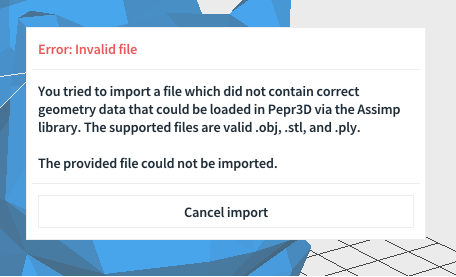
\includegraphics[scale=0.9]{images/invalid_file.png}
	\caption{Loading a file that does not contain any geometry will result in this error.}
	\label{fig:invalidfile}
\end{figure}

\begin{figure}
	\centering
	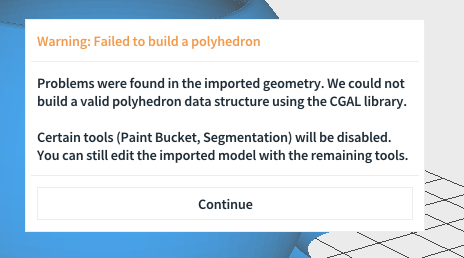
\includegraphics[scale=0.9]{images/polyhedron_failed.png}
	\caption{While this file could be loaded, the file does not conform to a certain assumption of some of the algorithms. Tools using these algorithms will be disabled, but the other tools will work correctly.}
	\label{fig:polyhedronfailed}
\end{figure}

\section{Coloring the model}

Once the model gets loaded, the user is free to select any available tools and color the model as he wishes. We have opted for a quick coloring of triangles, with all four colors. Our result is showcased in Figure \ref{fig:painted}.

\begin{figure}
	\centering
	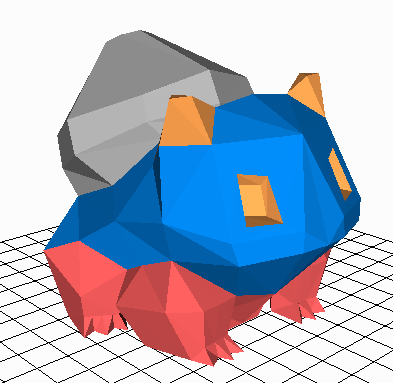
\includegraphics[scale=1]{images/result.png}
	\caption{Our demonstration coloring, achieved by using the Triangle and Bucket painters.}
	\label{fig:painted}
\end{figure}

\section{Exporting the model}

After we are happy with our coloring, we go to \textbf{File} -- \textbf{Export} and are presented with the user interface seen in Figure \ref{fig:exportui}. Here we select \textbf{TODO PARAMETERS}. We also select the checkbox to create a new folder for the exported files. After that, we select the volumetric export as multiple .STL files. A new folder is created, containing four different .STL files. We can now also save the project as the Pepr3D project file -- \textbf{.p3d}, in case we want to alter our coloring later.

\begin{figure}
	\centering
	
\includegraphics[scale=0.7]{images/export_ui.png}
	\caption{The demonstration of the Export GUI. Here we select the parameters mentioned in the text.}
	\label{fig:exportui}
\end{figure}

\section{Putting the files together in Slic3r}

In this section, we showcase how the parts we exported in the previous section look in the Slic3r application. In Figure \ref{fig:slicer}, the model is already loaded into Slic3r. This was done by loading one of the exported .STL files and then adding parts to it, in the \textit{Settings} menu of the object in Slic3r. We can now slice the model, and prove that the Pepr3D export worked correctly.

\begin{figure}
	\centering
	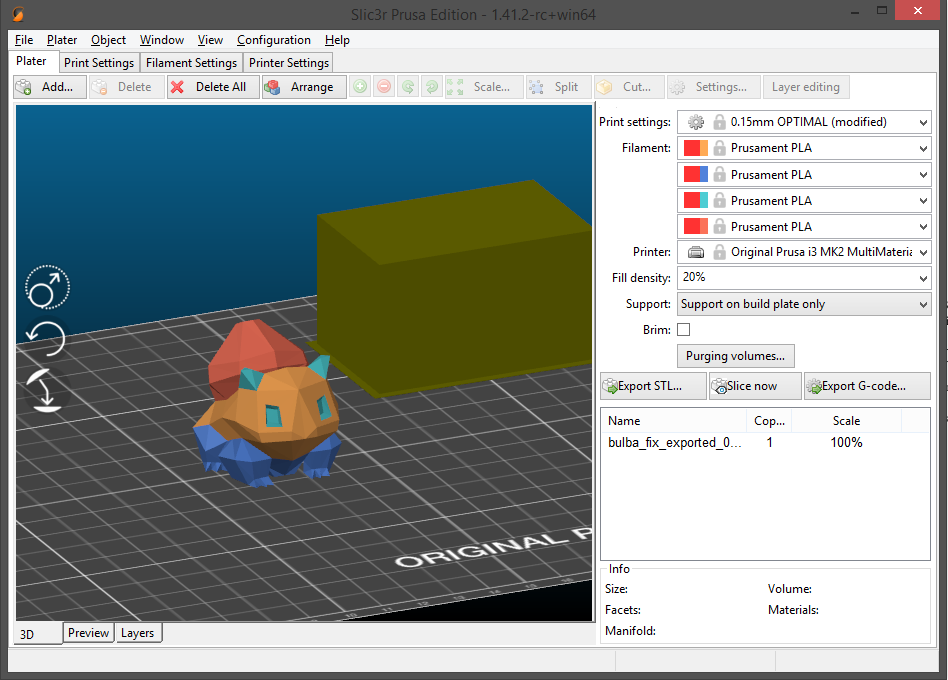
\includegraphics[scale=0.5]{images/slicer.png}
	\caption{The parts exported from Pepr3D loaded correctly into the Slic3r software.}
	\label{fig:slicer}
\end{figure}

\begin{figure}
	\centering
	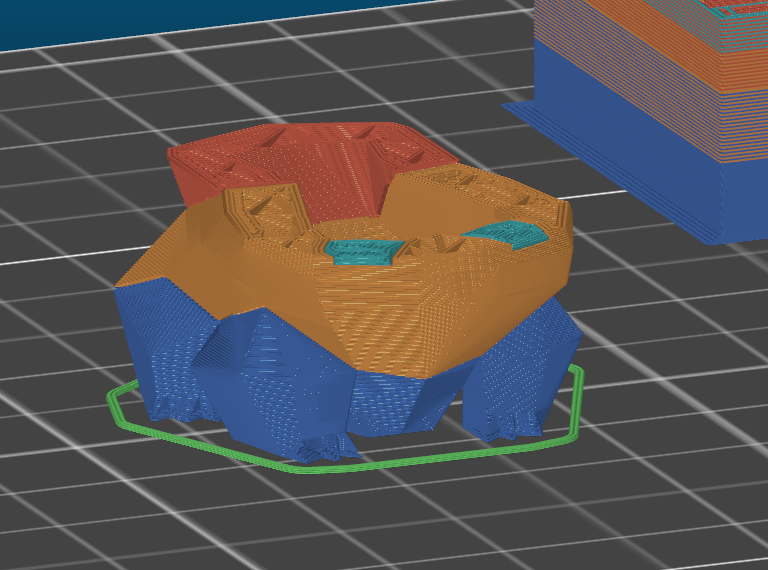
\includegraphics[scale=0.6]{images/sliced.png}
	\caption{The sliced, multimaterial model, ready to be printed.}
	\label{fig:sliced}
\end{figure}

\section{Printing the result}

After we are happy with the slicing we got, as shown in Figure \ref{fig:sliced}, we can print the model. We include several pictures of the printed result.

\begin{figure}
	\centering
	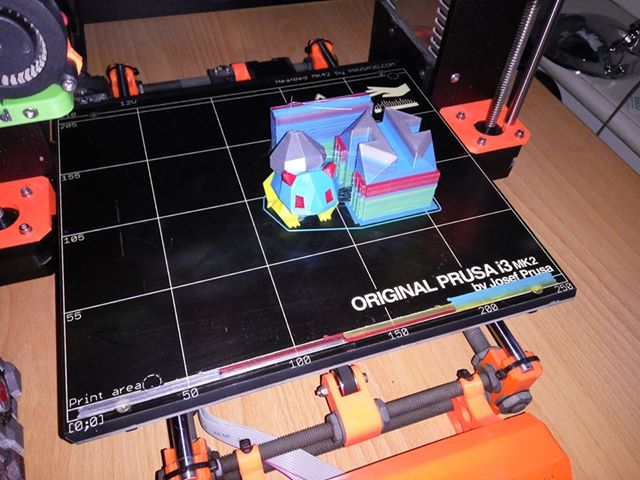
\includegraphics[scale=0.6]{images/printed_bulba.jpg}
	\caption{The printed model, with a custom wipe tower next to it.}
	\label{fig:printed1}
\end{figure}



% kritické zhodnocení přijatých řešení a možnosti dalšího vývoje
% 1. Chosen techniques critique - choosing CGAL/cereal/cinder, some other that didnt fit in their own chapter
% 2. Future work on the project - all that doesn't work and could, e.g. different more sophisticated export
\chapter{Conclusion}

In this chapter, we summarize the project, outline our experience with the 3rd party libraries that we have used, and elaborate on future work that can be done on the project.

\section{Summary}

In our software project, we aimed to design and fully implement an intuitive application for interactive colouring and exporting 3D models for 3D printing.
Within this documentation, we described the whole process behind this work together with our results.

We explained the basics of 3D printing and related works in Part I.
In Part II, we continued with a developer documentation describing our architecture and how we decided to implement the software.
Finally, here, in Part III, and especially in Chapters \ref{ch:min-req} and \ref{ch:results}, we prove that we have successfully fulfilled the goals and requirements initially set in our specification.

The whole application has been successfully verified together with our supervisor Oskár Elek and with our consultants Vojtěch Bubník from Prusa Research and Jaroslav Křivánek.
Possible future work that can be done together with Prusa Research is discussed later in this chapter.

\section{3rd party libraries}

Now we provide a quick summary of our experiences with the 3rd party libraries we decided to use.

\subsection{Cinder}

Cinder \footnote{https://libcinder.org/} is a C++ library which serves as a wrapper around OpenGL. It provides a multi-platform solution to creating an OpenGL window, handling keyboard and mouse input, simplifies the OpenGL buffer handling and much more. It is written with a modern C++11 standard and seemed like a good fit for our project.

Our experiences were mixed. On one hand, the library performed all the tasks we required and allowed us to spend little time worrying about Linux compatibility. On the other hand, the library itself forced a few very non-practical decisions on us, like the already mentioned C macro in the \texttt{main.cpp} file, which we discussed in Section \ref{sec:app}.

We also suspect, that the Cinder library is the main culprit behind our rather long compile times, since the problem existed basically from the beginning of the development, when the project did not include so much code.

\subsection{Dear ImGui}

Dear ImGui \footnote{https://github.com/ocornut/imgui} is a graphical user interface library for C++. We already discussed our reasons for choosing this library in the Section \ref{subsec:imgui}.

Our experience with this library has been very positive, as we have expected. The library is simple to use and simple to pick up. One of our team members was able to quickly start working with the library within a few days, without any prior knowledge. The limitation of this graphical user interface is the limited support for skinning, though this feature is not important at this time. It is difficult to use for an entirely custom user interface though, as some things are not yet exposed in the API, such as more advanced column layouts.

\subsection{CGAL}

The Computational Geometry Algorithms Library (CGAL) \footnote{https://www.cgal.org/} is the main library we chose to solve the geometry computations for this project, since it included several useful features, which we described in more detail in Chapter \ref{chap:geom}.

The team's experience with this library is conflicting. On one hand, the library performed everything we hoped for very well, did not raise many issues and we did not find any bugs, weird or wrong behaviour. On the other hand, the library is so heavily templated, that sometimes it is very hard to navigate. This problem is furthermore highlighted by its documentation, which is lacking in several places (with phrases like \texttt{Advanced feature.} as the only explanation to a public method). Since it looks to be generated from the code, the code does not provide any more information.

The members who have worked with the library were not satisfied with the library mainly for the user-friendliness, however, it is important to state that once you figure out the API and the general ideas behind the library, it performs well.

\subsection{Assimp}

Assimp \footnote{http://www.assimp.org/} is a library that handles importing and exporting of the models. This library holds a unique space in the C++ libraries for geometry loading and saving, because it is basically the only one which supports so many different formats for both importing and exporting. This makes it almost a must-include in a C++ geometry project and we hoped for an easy and fast integration.

In reality, we have had the most issues with Assimp out of all the libraries used. While the documentation is not plainly generated from code and explains a lot of concepts and ideas, it is not complete and the only thing left is reading the internal source code (not just the header files providing the API, the actual implementation as well). This happened several times during our development (while implementing post-processing during the import, while trying to use Assimp's progress reporters). Exporting a custom built scene (that did not get loaded by Assimp earlier), is only explained in the \textit{Issues} tab on Assimp's GitHub page, which also further highlights the lacking documentation.

We also encountered weird behaviour in the post-processing during the import phase -- we set Assimp to completely remove all degenerate triangles (triangles with an area equal to zero), which is described at length in Assimp's documentation. We found out that this pre-process, while configured exactly as the documentation stated, did not, in fact, remove all degenerate triangles, and we had to implement one additional check, after Assimp finishes.

In conclusion, while this library is the best on the market right now, it still has long ways to go, at least in our experience.

\subsection{Cereal}

Cereal \footnote{https://uscilab.github.io/cereal/} is a header-only library for (de)-serialization. The library has a minimalistic API and a solid documentation which explains all the major concepts behind it.

In our experience, it was very easy to pick up and add to our project and worked really well. So far we have not encountered any issues or found any bugs within the library. We have, however, discovered one limitation which the library imposes on the code it is used on. Any object which is to be loaded from serialized data either has to have a default constructor, or be stored by a pointer. If you have an object stored by value and it is not default constructible, the library will not know how to load it.

\subsection{Threadpool}

Threadpool library \footnote{https://github.com/progschj/ThreadPool} is a \emph{very simple} C++ library providing a simple threadpool. We used this library since we required a basic threadpool without too many features or overhead. This free code is simple, easy to check and functional.

\subsection{FreeType, FTGL and Poly2Tri and Font23D}

While doing research for the \textit{Text} tool on how to take a font file and a text string, and transform the bezier curves into triangle meshes, we found the \textbf{Font23D} library/project.

Font23D is a library/project on GitHub \footnote{https://github.com/codetiger/Font23D} without too much activity, but solving exactly the issue we faced as well. It incorporates the \textbf{Freetype}, \textbf{FTGL} and \textbf{Poly2Tri} libraries to solve the issue and we used it parts of this project in our own. You can read the exact development discussion about this library in Section \ref{sec:fonts}.

We made severe improvements and adjustments to the code from the repository, as the code is mainly written in \textbf{C}, instead of C++.

\subsection{Boost}

Last but not least is the Boost library which came as a pre-requisite for Cereal. Since we already had this library in the project, we decided we might as well use it. In the end, we did not use it for any major features but it was still handy to have around.

We will not discuss the quality of the documentation or the performance of this library, since it is a staple in the C++ environment.

\section{Future work}

In this section, we discuss the future work that could be done on this project. We divide the improvements that could be implemented into several categories:

\begin{itemize}
\item Improving existing core features
\item Adding \textit{quality of life} (QoL) changes to the GUI
\item Extending the toolset of the application
\end{itemize}

\subsection{Improving existing core features}

A few of Pepr3D's features and algorithms were developed by the team from scratch, since no solution satisfying our needs existed. These features are mainly the \textbf{Brush tool} and the \textbf{volumetric Export}. 

The brush tool uses computational geometry to subdivide triangles on the fly, which is not an easy task. Further work could be done by optimizing the brush tool to create better subdivisions and increasing the speed of the tool on bigger and more complex models. Our finished product is the best the team was able to come up with but with some more research, the tool can probably be optimized further.

The volumetric export (meaning the export which extrudes the faces inwards) is also a very complicated task, for which we have not found many solutions in any academic research or commercial products. We think that making this feature more robust would greatly improve the Pepr3D user experience.

\subsection{New quality of life features}

Since Pepr3D is a user-targeted application, the range of features the users have come to expect from the GUI of the program is vast. We implemented the basic subset of, what we think, are the most useful and important features -- such as hotkeys, tooltips and clear and simple user interface. However, there are many more features the users might benefit from, for example the radial menu around the mouse cursor, which we already discussed in Section \ref{sec:features}.

Other quality of life feature we got asked about by our colleagues during the development was a \textit{branching Undo \& Redo history}. This means that the command history would not be linear, but the user could go back a few commands from version B to version A, make new changes to version A, which would take him to version C. He could then compare versions B and C, which are both based on A and decide which he likes better.

The export GUI could additionally benefit from a tighter integration with 3D printing slicers. They could show the user in real time how the exported segments will look like layer by layer after being sliced for 3D printing. Our current visualization is not as advanced as we do not have the necessary data and algorithms for actually slicing the objects. This would make exporting the objects faster as users would not need to run another application.

\subsection{Extending the toolset}

When we designed the application's architecture, we put strong emphasis on allowing a potential developer to extend the toolset by adding other tools. We think we achieved this goal very well, because several of the tools require the same Geometry and Command API, which means we could add the tools and extend the functionality without implementing any additional functionality into Geometry or adding new Commands. This is the intended behaviour for the potential future developers.

If the new tool should require extending either the Geometry or Commands API, we strived to make the code educational -- if you need to create another command, you can read through one or two existing commands and then have a good understanding of how you should create your own.

% IV. USER DOCU
\addcontentsline{toc}{part}{Appendix: User Documentation}
\part*{Appendix: User Documentation}

% Podrobný popis instalace díla včetně přesné specifikace požadavků na použitý hardware a software
\chapter{System requirements and Installation}

In this chapter we will describe the system requirements of Pepr3D and the installation process.

\section{System requirements}

We divide the system requirements into \textbf{must have} items and recommended ones. The \textbf{must have} requirements are the following:

\begin{enumerate}
\item a 64-bit CPU with SSE instructions
\item a GPU supporting OpenGL version 3.2
\end{enumerate}

These two requirements are mandatory and Pepr3D might not work if you do not meet one or both of these.

Now we mention recommended system parameters. These are derived from what the team has been developing the software on, since we do not have an access to any larger data.

\begin{itemize}
\item \textbf{System:} Windows 8 / 10 (64-bit)
\item \textbf{Processor:} Intel CPU with clock speed 2.0 GHz or higher, 2 or more CPU cores and 64-bit and SSE instructions
\item \textbf{Memory:} 2 GB or more
\item \textbf{GPU card:} GPU card compatible with OpenGL 3.2
\item \textbf{Storage:} 200 MB
\end{itemize}

\section{Installation}

Installing Pepr3D is very easy. After downloading the compressed archive, unpack it into a folder anywhere on your hard drive. Pepr3D should now be ready to run.

% Showing the tool for the first time to a new user
\chapter{First run}

In this chapter we show the usage of Pepr3D for complete beginners. It covers every step from starting Pepr3D to exporting a simple colored model including importing, manipulating and using tools.


\section{First look at Pepr3D}

When you run Pepr3D, you will see a cube at the center of the application. There is a toolbar at the top of application which contains file menu, undo/redo buttons, set of tools and some settings. There is also a side pane on the right with settings of individual tools as you can see in figure \ref{fig:pepr_cube}.

\begin{figure}
	\centering
	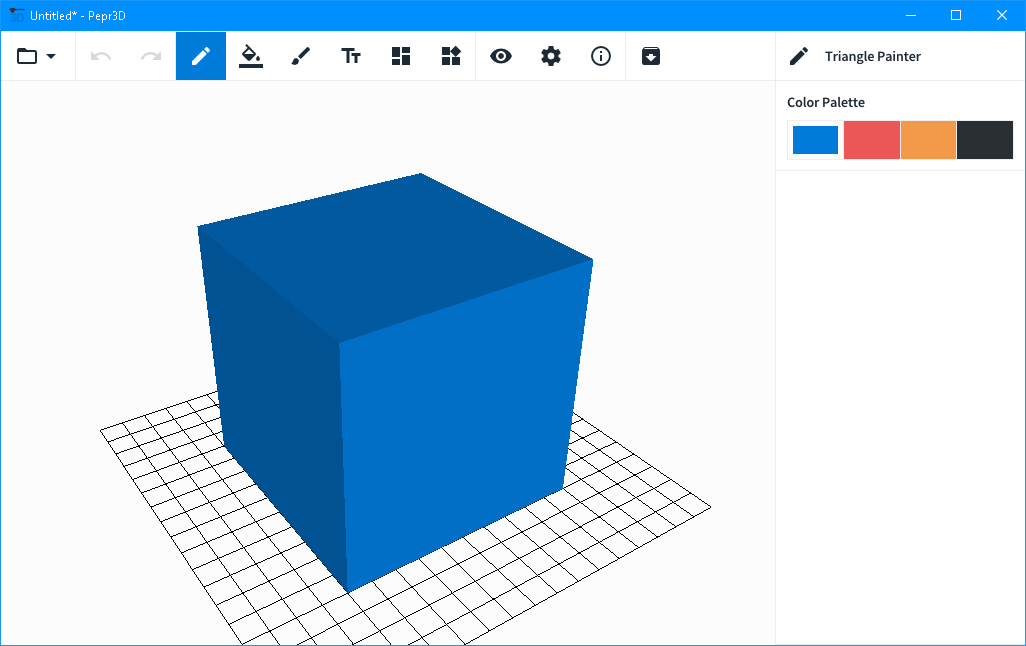
\includegraphics[scale=0.5]{images/pepr_cube.png}
	\caption{Pepr3D appearance after start-up.}
	\label{fig:pepr_cube}
\end{figure}

\subsection{Model manipulation}
You can manipulate the model by using your mouse. There are several ways to manipulate so you can reach and see any part of the model:

\begin{itemize}
\item \textbf{Rotation} -- Click and hold right mouse button and move.
\item \textbf{Translation} -- Press Ctrl + right mouse button and move, or press and hold the middle mouse button (mouse wheel) and move the mouse.
\item \textbf{Zoom} -- Scroll with the mouse wheel.
\end{itemize}

Left mouse button is dedicated to using selected tool.

\section{First model}
Now we can start working on a simple model with Pepr3D. First we have to acquire a 3D model, it should be in one of these file formats: \texttt{.stl}, \texttt{.ply}, \texttt{.obj}. The simplest way to acquire model is choose any model on the internet and download it. Or you can use any 3D modelling software and create one on your own. In this tutorial we use a simple low-polygon model of a Bulbasaur downloaded from Thingiverse\footnote{https://www.thingiverse.com/thing:327753}.

To import the model we can use a drag and drop gesture with the model file or we can browse for a model file after clicking \textit{Import} in the file menu.


\subsection{Painting the model}

After importing the model we can use any tool that our application provides to color the model as we want. In a few steps, we will show how to quickly color the imported model of our Bulbasaur with basic tools.

\begin{enumerate}
\item Select the \textit{Triangle Painter} tool, choose black color in the color palette.
\item Paint all triangles in each eye by clicking on them with the left mouse button. It is possible to click and drag to paint multiple adjacent triangles at once.
\item Use the same technique to paint its ears.

\begin{center}
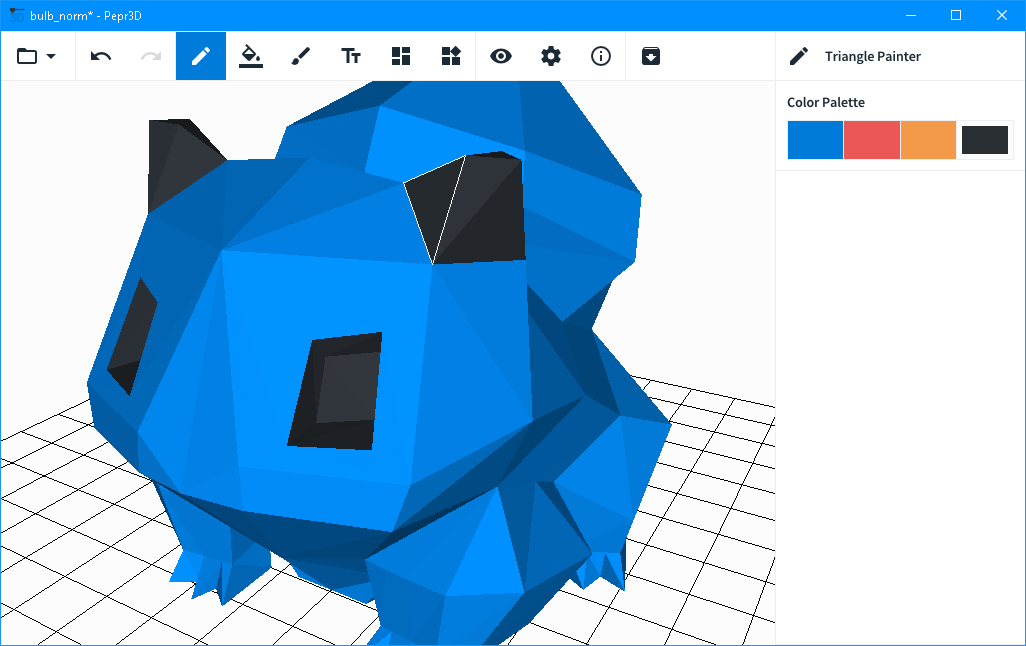
\includegraphics[scale=0.4]{images/bulb_eyes.png}
\end{center}

\item Choose another color (red) and select the \textit{Paint Bucket} tool.
\item Check \textit{Stop on sharp edges} in the side pane and set the \textit{Maximum angle} to 45$^\circ$.
\item Use the \textit{Paint Bucket} on any triangle on the "onion" on the back of the Bulbasaur. Click two more times on any unpainted triangle to paint the whole "onion" with red color.
\item Select the \textit{Triangle Painter} and the first color (blue) and recolor two triangles near the neck which have been painted extra by the \textit{Paint Bucket} in the previous step.

\begin{center}
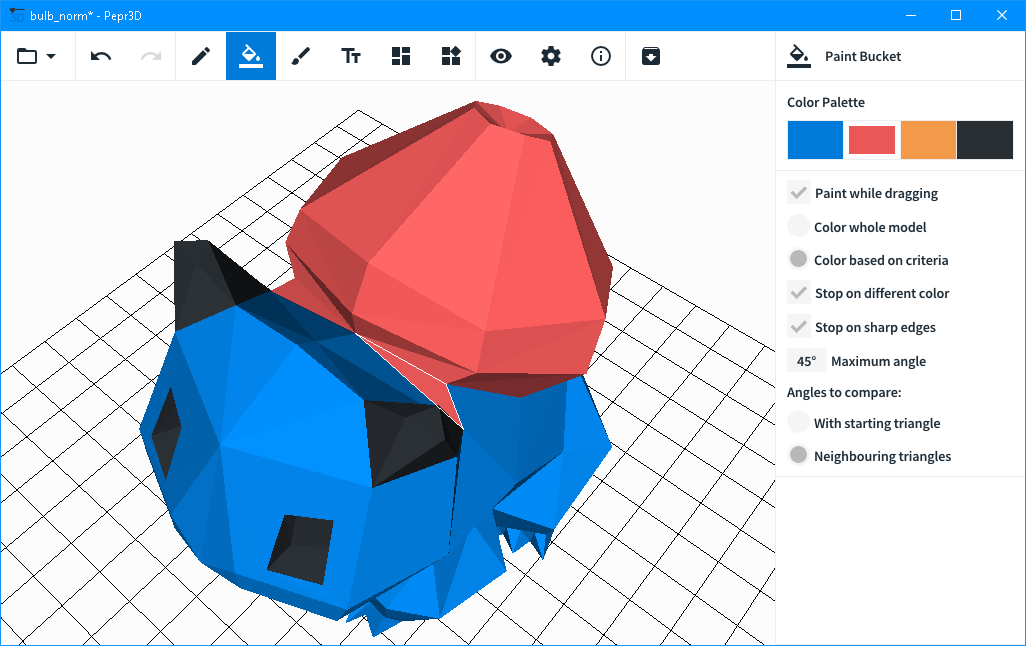
\includegraphics[scale=0.4]{images/bulb_onion.png}
\end{center}

\item Select the \textit{Brush} tool and check both the \textit{Respect original triangles} checkbox and the \textit{Paint outer ring} checkbox in the settings of the tool.
\item Set the brush size to about 4.0.
\item Choose orange and paint each leg. Do not forget to paint the legs from below.

\begin{center}
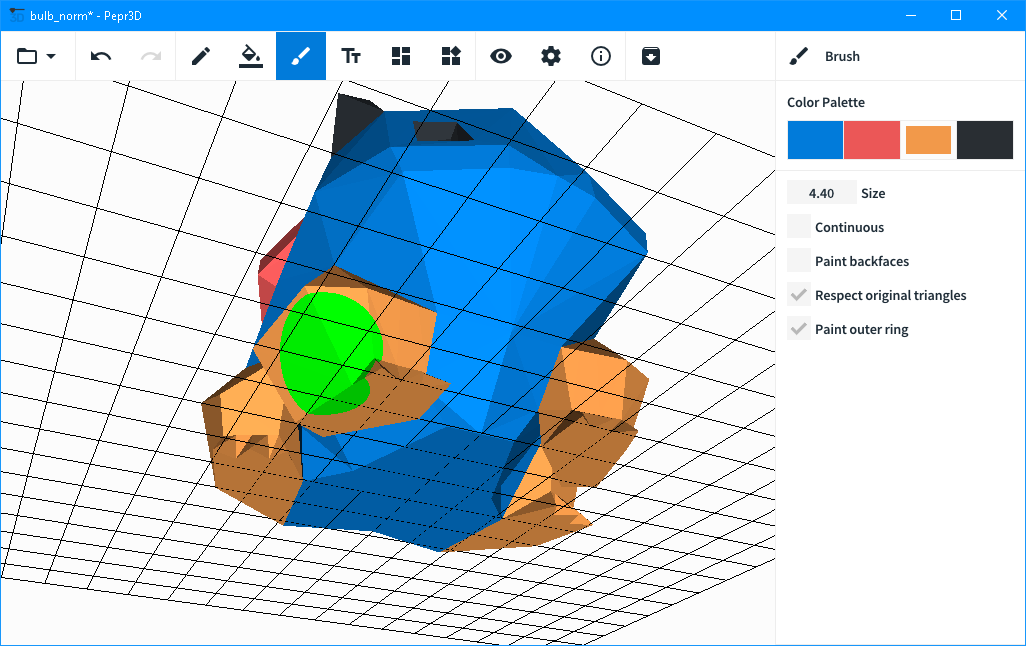
\includegraphics[scale=0.4]{images/bulb_legs.png}
\end{center}

\end{enumerate}


You can undo any step you did with any tool. For example, if you paint on a incorrect triangle, you can press \textit{Undo} (left arrow) in the toolbar to revert the mistake.

\subsection{Exporting the model}
Now the model is painted and we can proceed to model exporting. Before exporting the model itself we need to set the depth of color extrusion into the model. Exporting can be summarized in the following steps:


\begin{enumerate}
\item Open the \textit{Export Assistant} on the toolbar or click \textit{Export} in the file menu.
\item Click the \textit{Update extrusion preview!} button.
\item Lower the percentage of \textit{Max Preview height} to see into the model and see the thickness of model walls -- the extrusion depth.
\item Adjust the percentage of \textit{Depth} for the desired extrusion depth.
\item Update the preview by clicking on the \textit{Update extrusion preview!} button.
\item Repeat adjusting the depth and updating the preview until you are satisfied.
\item Click on \textit{Export files} and complete the export.
\end{enumerate}

\begin{figure}
	\centering
	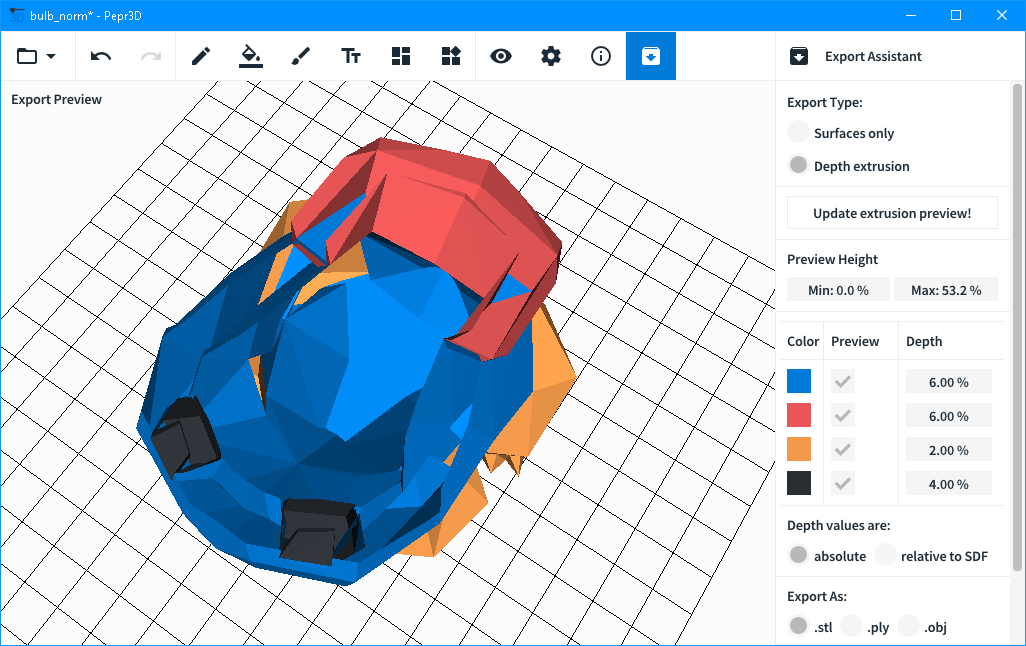
\includegraphics[scale=0.5]{images/bulb_export.png}
	\caption{Example of \textit{Export Assistant} with colored model.}
	\label{fig:bulb_export}
\end{figure}


Exported files can be now imported into any supported slicer and printed on a multimaterial 3D printer.






% Demonstrate and explain each tool to the USER (not a software guy)
\chapter{Tools}

This chapter covers all the tools the user has at his disposal. We explain each tool's purpose and all the parameters the user can set.

\section{Triangle Painter}

Triangle Painter is the simplest tool of Pepr3D. It allows the user to color a single triangle with a selected color. This can be performed either by a single click on the model's triangle or by dragging the mouse over several triangles with the left mouse button pressed down.

The triangle that is currently hovered (has the mouse cursor over it) will be highlighted on the model's surface with a different border color.

The only property the user is able to select in this tool is the current color from the color palette.

Pressing the \textit{Undo} will undo the last stroke of the triangle painter. This means it will undo \textbf{the whole} stroke, if the user dragged the mouse over several triangles.

\section{Bucket Painter}

Bucket Painter is a simple tool that can be used to achieve sophisticated results easily. This tool works as one is used to from image editing software like GIMP \footnote{https://www.gimp.org/} or Adobe Photoshop \footnote{https://www.adobe.com/products/photoshop.html} -- it starts colouring every triangle it can reach, starting with the triangle the user clicked on.

\subsection{Properties}

The properties of this tool revolve around the spread of the bucket. This is something we call \textit{stopping criteria}. We now list all properties of the tool and explain each one in detail.

\begin{itemize}
\item \textbf{Color Palette} -- This widget allows the user to select the current active color. The selected color will be spread by the bucket. Customizing the palette can be performed in the \textit{Settings} panel.

\item \textbf{Paint while dragging} -- \textit{On / Off} -- This checkbox specifies whether the bucket painter will only function by clicking on single triangles (\textit{Off}) or will bucket spread continuously if the user drags the mouse in a stroke (\textit{On}). We recommend leaving this \textit{On} unless it disrupts you or the model you are working on is very big.

\item \textbf{Color whole model} -- \textit{On / Off} -- We have mentioned \textit{stopping criteria} in the beginning. This is the  first choice the user can make that affects the stop of the bucket spread. If the user selects this option, the Bucket Painter will simply color the whole region of the model. If the model is a single mesh, it will color the whole model. Turning this \textit{On} will hide the other options. Turning this \textit{Off} allows the user to specify the \textit{stopping criteria}.

\item \textbf{Stop on different color} -- \textit{On / Off} -- The simplest \textit{stopping criterion}. The spread will only re-paint triangles which have the same color as the triangle the user clicked on. Additionally, the spread will stop if a new color is met. If this is the only criterion that is enabled, the Bucket Painter will work exactly as we are used to from image editors. This is the default setting of the tool.

\item \textbf{Stop on sharp edges} -- \textit{On / Off} -- A second \textit{stopping criterion} which can be enabled or disabled. Enabling it expands the user interface to allow the user to modify the criterion. This criterion will not care about the color the user clicked on, and only stops from spreading to the neighbouring triangle, if the neighbouring triangle is at a greater angle than specified. The exact behaviour is specified by the following properties.

\item \textbf{Maximum angle} -- \textit{$0\degree$ -- $180\degree$} -- Specifies the angle which the two neighbouring triangles have to be angled at for the bucket painter to stop spreading. If the angle between the two triangles is greater than this value, the spread will not color the triangle and will stop.

\item \textbf{Angles to compare} -- \textit{With starting triangle / Neighbouring triangles} -- the last choice in the sharp edges \textit{stopping criterion}. If the user selects \textit{With starting triangle}, the angle will be measured between the triangle the user clicked on and the triangle currently being coloured. For example, if this option is chosen, the angle is set to $95\degree$ and a single face of the cube is clicked, all faces of the cube except the opposite one are coloured. This is because the opposite face is at an $180\degree$ angle. If the user selects \textit{Neighbouring triangles} and uses the $95\degree$ setting again, the whole cube will get coloured, because there are no faces on the cube that are at an angle greater than $95\degree$.

\end{itemize}

Both of the \textit{stopping criteria} can be selected together. The spread stops when one of the criteria is not fulfilled -- both of the criteria must be fulfilled for the spread to continue.

\section{Automatic Segmentation}

Automatic segmentation is a powerful tool which allows the user to quickly achieve the baseline colouring of the model, which then can be detailed to the user's liking. This is achieved by separating the model into several segments based on the thickness. These segments then can be quickly coloured individually. The user can select the sensitivity of this segmentation, which allows him to control the level of detail (for example, low sensitivity might only segment the body and limbs of a character, whilst high sensitivity will also segment the fingers, ears and horns).

\subsection{Properties}

\begin{itemize}

\item \textbf{Compute SDF values} -- \textit{button} -- before anything can be done in this tool, the user is asked to compute the SDF values. This is the data that is required to perform a successful segmentation. This computation might take a long time to perform, depending on your model size. For low-poly models (e.g. 1000 triangles), this computation is instantaneous. If you already performed the computation in a different tool (like export or the other segmentation), this option will not be visible.

\item \textbf{Segment!} -- \textit{button} -- this button starts the segmentation process. The default values are set so the segmentation returns viable results in most cases. If you did not set any of the following properties and the segmentation returned an undesirable number of segments (like only one or too many), modify the following properties.

\item \textbf{Robustness} -- $0\%$ -- $100\%$ -- a magic parameter. The meaning of this parameter is somewhat obscured but the best way to imagine this setting is the quality or robustness of the segmentation. Higher values take longer to compute but might give better results -- a higher value might merge two segments that are somewhat related, which the lower values will not recognize. The default setting is the team's best effort to balance the performance and quality.

\item \textbf{Edge tolerance} -- $0\%$ -- $100\%$ -- This parameter specifies how the algorithm should understand "thickness". If you set this value very high, the algorithm will tend to merge more segments together, resulting in a lower amount of segments. If you set this very low, every nook and crease will signal the algorithm to create a new segment, thus resulting in a higher amount of segments. This is the \textbf{primary means} to control this tool and we recommend adjusting this slider over the previous one to change the main behaviour.

\item \textbf{Color Palette} -- same as in the previous tools, this widget allows the user to select a color to assign to each segment.


\end{itemize}

\subsection{Segmentation}

To adjust the segmentation, we recommend first trying to adjust the \textit{Edge tolerance} slider, and only after experimenting with this slider to change the \textit{Robustness}.

After these settings are adjusted and the user clicks on the \textit{Segmentation} button, a list of segments will appear, along with the number of segments created. The user is then instructed to assign a color from the color palette to each segment. This can be done in two ways -- either by clicking directly on the model or by clicking on the "Segment \#" button. After clicking on one of these two regions, the color selected in to color palette will get assigned to the segment.

After \textbf{all segments} have been assigned a color from the color palette, the user is able to click \textit{Accept} to color the model this way. Should the user be dissatisfied with the colouring, he can either click \textit{Cancel} or \textit{Segment!} again, to completely undo the whole segmentation and start from scratch.


\section{Manual Segmentation}

Manual segmentation is a similar tool to the Automatic segmentation we discussed in the last section. The difference in these two tools is that while Automatic segmentation is a very global tool (since it segments the whole model at once), Manual segmentation is designed to be local. The user can color a handful of triangles with a single color and then manually adjust the spread of this color over the segment the triangles define. This description is rather abstract, but hopefully it will get clearer once we discuss the properties.


\subsection{Properties}

\begin{itemize}

\item \textbf{Compute SDF values} -- \textit{button} -- before anything can be done in this tool, the user is asked to compute the SDF values. This is the data that is required to perform a successful segmentation. This computation might take a long time to perform, depending on your model size. For low-poly models (e.g. 1000 triangles), this computation is instantaneous. If you already performed the computation in a different tool (like export or the other segmentation), this option will not be visible.

\item \textbf{Color palette} -- once SDF values of the object have been computed, the user is presented with a sidepane very similar to the Triangle painter tool. This widget allows the user to select the current color. The color will be used while initializing the segments on the model.

\item \textbf{Spread} -- $0\%$ -- $100\%$ -- once a single triangle is coloured on the model, additional options appear. One of them is the \textit{Spread} slider. This slider is analogous to the \textit{Edge tolerance} slider in Automatic segmentation, since it controls how much each coloured triangle will spread its color among its local neighbourhood. If the spread is $0\%$, only the triangle is coloured. Increasing it to $100\%$ will color all triangles of the model (unless a second segment is competing).

\item \textbf{Hard edges} -- \textit{On / Off} -- if this option is turned on, the spread of one color will stop upon meeting a second one's border and will not attempt to color any other triangles. Use this option if the segments you are colouring are well defined and differ in thickness a lot.

\item \textbf{Region overlap} -- \textit{On / Off} --once the user turns this option on, the spreading regions will overlap freely and the last color (rightmost) will always win if \textit{Spread} is turned to $100\%$. Use this option if the borders of the segments converged a little soon or late and you would like one color to expand a little more. This option is not good if the spread is turned to high percentages, since a lot of the segments will overlap and information will be lost.

\end{itemize}

\subsection{Segmentation behaviour}

If no checkboxes are turned on, the color spreads to the global optimum segmentation. This means that if you set the \textit{Spread} to a high percentage, there might be several discontinuous segments coloured by the same color, because that is globally optimal to the input. This setting is a good starting point, since it does not restrict the spread too much, but does not allow it to roam unlimited as well. Use the other options to tweak the spread after you understand how this model will get segmented.

The spreading algorithm uses the SDF function (thickness of the model) to calculate segments. This means that this tool is not able to grow segments on a model which does not vary in thickness. It is also very important to be aware of the fact that several non-neighbouring parts of the model might have the same thickness (like ears, hand fingers and feet fingers) and thus the global optimum colors all of these with the same color (use \textit{Hard edges} to counter this behaviour).

After the user is satisfied with the spread, clicking \textit{Apply} will confirm this re-colouring. Clicking cancel will return the model into the state before Manual segmentation started.

As a last tip, we recommend using a single-triangle strokes to initialize the segments at the beginning. This is using many triangles accelerates the spread a lot, which ultimately gives the user less fidelity and time to see what is happening.

We want to stress that this tool is an advanced tool, which should be used to fine-tune an already coloured model's details, not as a means to primarily color the model upon importing it (Automatic segmentation is a lot better tool in that case).

% Demonstrate export and import, maybe even with SLICER support
\chapter{Import, Export and Saved projects}

In this chapter we explain in-depth how the users should import their models, all the different methods of exporting their work and the ability to save their work as a \textit{Pepr3D project} to continue at a later date.

\section{Importing a model}

Importing the model is the first step in the Pepr3D workflow. There are several ways how to import a model and all of them are equally easy and the choice is entirely up to you.

\begin{enumerate}
\item \textbf{File} $\rightarrow$ \textbf{Import} will open a typical \textit{Open} dialog of you respective operating system. Navigate to the model you want to import and click the button \textit{Open}.

\item \textbf{Drag and drop} is a very fast way to import the model if you already have it located in any file explorer. The model can be dropped into any part of Pepr3D.

\item \textbf{Control + I} is the keyboard shortcut for importing a model. Upon pressing this shortcut, the \textit{Open} dialog of you respective operating system will open. Navigate to the model you want to import and click the button \textit{Open}.

\end{enumerate}

After you perform either of the two previous steps, the model will start loading. There is a detailed dialog which explains what is currently happening and Pepr3D is trying to give you accurate information about the progress of the process. However not every computation has a well known length, so several loading bars will just cycle through until the loading is complete. Please be patient, loading a large model can take a long time. See Table \ref{tab:loadperf} for a rough idea about the loading times.

\begin{table}[]
\centering 
\begin{tabular}{|c|c|}
\hline
\textbf{File size {[}MB{]}} & \textbf{Estimated loading time {[}s{]}} \\ \hline
80                          & 3                                   \\ \hline
15                          & 2                                   \\ \hline
5                           & 1                                   \\ \hline
1.2                         & 0.5                                 \\ \hline
\textless{}1                & \textless{}0.5                      \\ \hline
\end{tabular}
\caption{Loading times during the import into Pepr3D.}
\label{tab:loadperf}
\end{table}

\section{Exporting a colored model}

When you finish painting a model in Pepr3D and you would like to use it in 3D printing or another application, it is necessary to \emph{export} the colored model.
This saves your work to files which are compatible with other software.
To be more precise, 3D printing a model with different colors typically requires separate colors in separate files, which exporting in Pepr3D does.

To export a model you have painted in Pepr3D, use our \textbf{Export Assistant}.
You can access it by clicking on its \textbf{icon in the Toolbar}, by using the default hotkey \textbf{Ctrl + E}, or from the File menu \textbf{File $\rightarrow$ Export}.

Once you select the Export Assistant, you can change its options in the side pane.
On the left side, a preview of the export will be shown, but only for certain options described later.

In the side pane, as the very first decision, you can choose between exporting \emph{only the surfaces}, or exporting with \emph{depth extrusion of the colors}.
As these two options influence the rest of the export process, we describe them separately in the following subsections.

\subsection{Exporting surfaces only}

Exporting only surfaces of your painted model is the simplest option.
All triangles with the same color are grouped together and saved to a separate file.
The result are multiple files containing the differently colored surfaces of the model.

This option is useful when you want to use your painted model in another 3D editor such as Blender.
It is not entirely useful for 3D printing as common slicers are not capable of actually printing these exports reasonably.
That is because volumetric information, i.e., how deep the colors should be extruded, is missing in this export.

The only options in the side pane are the file formats and then a simple \textbf{``Export files''} button which opens a file dialog to save the files.
Follow Section~\ref{sec:exportformats} for more details.

\subsection{Exporting extruded colors}

Unlike surface export, extrusion export has various options and also provides you with a preview of the options.
The biggest difference is that extrusion export is much more suitable for 3D printing as it provides volumetric information, i.e., how deep the colors should be extruded.
The user can specify this extrusion information in the various options.

At any time you can press the \textbf{``Update extrusion preview!''} button and a preview of the export will be shown on the left side of the Pepr3D window.
The point of the preview is so that you as the user can see how the model is going to look like after being exported.
Generally, the preview should look exactly as the model you painted, unless there are errors and the options are wrong.

By changing the range in the \textbf{``Preview Height''} option, you can see inside the model.
Raising the minimum height removes a bottom part of the model.
Lowering the maximum height removes an upper part of the model.
This only affects the preview, not the actually exported files!

Being able to see inside the model is very useful in extrusion export, as it helps you understand how deep the colors will actually penetrate.
One of the most important things to remember is that the extrusion \emph{should never penetrate} the original surface!
If the extruded part penetrates the surface on the opposite side, you have to lower the depth of that color!

This can be done by changing the \textbf{``Depth''} in the table of colors.
The depth percentage is with regards to the size of the object, where $100\%$ corresponds to the size of the whole object.
This means that if you set an extrusion that high, it will almost for sure penetrate the surface and be wrong.
We should always operate with lower extrusion depths such as a few percent only.

In models that have SDF (shape diameter function) values available, you can set the depths to be \textbf{``relative to SDF''} instead of ``absolute''.
This is very useful for complex models with varying thickness, e.g., models with spikes, little details, etc.
Relative depths are not only based on the percentage you set, but they also vary locally with regards to the local thickness of the model.
So for a certain color and percentage you set, the depth will be \emph{higher} than your percentage in thick parts of the model and \emph{lower} in thin parts of the model.
This is different than in ``absolute'' thickness where all triangles are extruded the same.

To verify how the extrusion looks inside the model, you may also disable the \textbf{``Preview''} of certain colors in the table of colors.
This will simply hide all triangles and extrusions of a certain color from the preview, but not from the exported files that you actually export.

The export is finished using the \textbf{``Export files''} button (see Section~\ref{sec:exportformats}).

\subsection{Advice for 3D printing}
When exporting for 3D printing, try to follow the following recommendations:

\begin{itemize}
\item Always use the \textbf{``Depth extrusion''} option unless it gives completely wrong results with whatever extrusion options you try. In that case, it might be necessary to use \textbf{``Surfaces only''} and do the extrusions manually in a 3D editor such as Blender.
\item Make sure the extruded parts never penetrate the object surface from the opposite side. This penetration will be visible in the 3D printing! If that happens, make sure to lower the \textbf{``Depth''} of that color. On the other hand, too low depths may be impossible to print as the model would be too hollow. It is necessary to find the right balance.
\item For certain slicers such as Slic3r Prusa Edition, the extrusions \emph{may} intersect in the interior of the model. The slicer will fix this automatically when generating the G-code for printing.
\item In models with various thickness in different parts, e.g., models with spikes, little details, etc., try to use depths \textbf{``relative to SDF''}.
\item If parts of a model with a certain color are too deep or too shallow but changing the percentage for the whole color breaks in another part of the model, consider adding a new color to the palette. You can paint the two parts with different colors but still print them with the same color! Remember that in the 3D printing slicers, you can set multiple parts from Pepr3D to be printed with the same color. \textbf{The Pepr3D color palette does not have to correspond to the colors you actually print!}
\item If you want a part of a model to be filled instead of partially hollow, you can \textbf{experiment by setting a color depth to $0.00\%$}. This will not extrude it at all, so certain 3D slicers such as Slic3r Prusa Edition will try to fill in the parts completely! You can verify this when you import the exported files to the slicer and preview the layers.
\item Always verify the extrusion by importing the exported files to a slicer, generating the G-code, and previewing the model layer by layer, if it is supported by the slicer.
\end{itemize}


\subsection{Supported formats}
\label{sec:exportformats}

When exporting the files, before clicking on the \textbf{``Export files''} button which opens a file dialog to save the files, there are options to choose from.
First, you can choose from 3 file formats described below.
Then, you can also check the \textbf{``Create a new folder''} option, which means that a new folder will be created and all the exported files will be saved in the new separate folder (directory).
This is useful when using multiple colors and neatly organizing your exports.

The supported file formats are:

\begin{itemize}
\item binary \textbf{.stl} (stereolithography) files, they are suitable for example for 3D printing with Prusa printers and Slic3r Prusa Edition,
\item binary \textbf{.ply} (Stanford Triangle Format) files, they are supported by common 3D editors,
\item non-binary \textbf{.obj} files that are also saved with their corresponding \textbf{.mtl} files, also supported by common 3D editors.
\end{itemize}

\section{Saving and opening a project}

\subsection{Saving a project}

Saving a project to work on it later is very simple in Pepr3D. There are two save options in Pepr3D:

\begin{enumerate}
\item \textbf{File} $\rightarrow$ \textbf{Save} will overwrite your last save file with the current state of the model. If you have not yet saved the project at all, this option also acts as \textit{Save As}. The keyboard shortcut for \textit{Save} is \textbf{Ctrl + S}.

\item \textbf{File} $\rightarrow$ \textbf{Save As} will prompt you with a \textit{Save As} dialog of your respective operating system. Upon selecting the folder and choosing the name, the project will be saved inside the folder with the chosen filename. There is no keyboard shortcut for \textit{Save As}.
\end{enumerate}

If your project has been modified since the last save, you will see an asterisk (*) next to the project's name.

Please note that Pepr3D \textbf{does not} save your work undo history. If you save a project and re-open it, you \textbf{will not} be able to undo any operations done by the previous session.

\subsection{Opening a project}

Opening a project can be done through \textbf{File} $\rightarrow$ \textbf{Open} or simply by pressing \textbf{Ctrl + O}. Both of these options will display the \textit{Open} dialog of you respective operating system. Here you can choose the \textbf{.p3d} file and press open.

Opening a project can also be performed by \textbf{drag and drop}. Simply grab your \textbf{.p3d} file and drop it anywhere into Pepr3D.

As we have mentioned in the section about saving projects, keep in mind that Pepr3D \textbf{does not} save your work undo history.


% Explain all settings - both view and program options
\chapter{Additional options and settings}

In this chapter, we showcase and explain all the preferences and settings Pepr3D contains. There are two main categories of the settings the user can alter in Pepr3D: \textbf{Display options} and \textbf{Settings}. \textbf{Display options} contains all settings regarding the displaying of the model and handling the camera. The \textbf{Settings} tab contains the important \textit{Color Palette} manager and some extra UI settings. We now discuss each category in more detail.

\section{Display options}

This tab of the interface contains all properties related to the user's view and interaction with the model. These preferences are divided into three segments and we will explain every one in detail.

\subsection{Camera zoom behavior}

This option provides the choice between two most common camera zoom behaviors, namely the \textbf{dolly} and \textbf{field of view}. Both of these are widely used in computer graphics and there is no clear consent on which of these two is better.

\begin{itemize}
\item \textbf{Dolly} -- as the short text next to the option explains, this setting physically moves the camera within the space of the program, while the field of view stays the same. This option is the default setting, since the zooming in and out is more intuitive because it replicates moving the observer's eye closer to the object. The disadvantage of this method lies in editing fine details on the surface. This is because the \textbf{dolly} allows the camera to enter the inside of the object, which means the user is not able to zoom as close as he might like.

\item \textbf{Change field of view} -- the second widely used option amongst the graphics editors. This option does not move the camera but only changes the field of view (FOV for short). This means the camera will never fly inside the object and is able to provide as close of a look as the user desires. The main disadvantage of this approach is slightly worse handling when zoomed in really close.

\item \textbf{Reset camera} -- a simple button to reset the camera to the default position. This is the position the object appeared in after the model import was done.

\end{itemize}

Feel free to change this camera zoom behavior to the one you like, it does not affect the performance or model quality in any way.

\subsection{Model transformation}

While Pepr3D tries to orient your model correctly from the start, it only succeeds if your model follows the Blender axis alignment. This is the \textbf{X left-right, Y forward-backward, Z down-up} axis alignment. This is the most common spread axis system and is the one Pepr3D supports without any adjustments. This is the axis system that Prusa Slic3r uses, so if your model works in Slic3r, it should natively work in Pepr3D. Should you need to use a different system, this segment of the settings provides you with means to correct for this change manually.

\begin{itemize}

\item \textbf{Model roll} -- $0\degree$ -- $180\degree$ -- If the model is incorrectly oriented, you can rotate the model with this slider. You can control the camera with the right click drag, which rotates the camera in two axes around the model. This option rotates the model along the third axis, which allows you to fully customize the object's orientation. If your model is incorrectly oriented, this slider should always be able to fix the issue.

\item \textbf{Model position} -- $-1.00$ -- $1.00$ in X/Y/Z axes -- Pepr3D tries to center your model onto the guiding grid. Should Pepr3D not succeed, these options allow you to position the model correctly.

\item \textbf{Reset model transformation} -- \textit{button} -- a simple button to reset the model to the default position. This is the position the object appeared in after the model import was done.

\end{itemize}

\subsection{Guidance graphics}

The last section contains a couple of guiding tools that the user might want to use to help his orientation in the space or understand the model's geometry better.

\begin{itemize}

\item \textbf{Show grid} -- \textit{On / Off} -- determines whether the model should be positioned on a guiding grid or not. This is done to simulate the printing bed of the 3D printer itself. It also should help the user with orientation, if the model is symmetrical.

\item \textbf{Show wireframe} -- \textit{On / Off} -- if enabled, every triangle on the model will have its borders displayed in a high contrast color. This option is turned off by default since it is distracting on complex models but might be a really useful tool to see how the model geometry looks like and how it got changed by the Brush or Text tool.

\end{itemize}

\section{Settings}

For now, there are only a couple options in the Settings menu. They are, however, very important to understand.

\subsection{Editing the color palette}

This is probably the most important setting in Pepr3D, because it affects every tool and the outcome of the export. Here you can \textbf{add or remove} additional colors into the palette, \textbf{change} the already existing colors, as well as \textbf{reorder} them or \textbf{reset} them into the default stage. Let's talk about these options in more detail.

\begin{itemize}

\item \textbf{Add color} -- \textit{button} -- adds a new color into the palette. The hue of the color is randomized. See \textit{changing the color} to learn how to change the hue. The maximum number of colors for now is \textbf{16}, since the most advanced FDM printers cannot print more than that many colors.

\item \textbf{Delete color} -- \textit{drag and drop field} -- deleting a color is as simple as grabbing it and dragging it onto the red zone with the \textit{Drag color here to delete} description. Be careful, since this \textbf{will permanently delete} all information associated with the color. Any triangles painted by this color will get a new color (the previous one in the palette). This operation \textbf{is undoable}.

\item \textbf{Reordering the colors} -- \textit{drag and drop within palette} -- you can rearrange the colors by dragging and dropping them accordingly. Note that this \textbf{does not change} the colouring of the model and is \textbf{only cosmetic}. This operation \textbf{is undoable}.

\item \textbf{Changing one color} -- \textit{right click on the color} -- if the user wishes to change the the color, it is done by left-clicking the color patch. Once clicked, a color picker gets displayed and the user can change the color there. Note that this \textbf{does change} the color on the model in real time, which allows the user to preview the change. This operation \textbf{is undoable}.

\item \textbf{Resetting colors to the default values } -- \textit{button} -- once clicked, the colors will be reset into the default values and the model will be re-coloured according to the positions of the first four colors. This operation \textbf{is undoable}.

\end{itemize}

\subsection{User interface preferences}

This section allows the user to modify the appearance of the Pepr3D software.

\begin{itemize}

\item \textbf{Side pane width} -- \textit{in pixels, relative to Pepr3D's width} -- this modifies the width of the side pane area. This is especially useful if the user is working with more than four colors or on a high resolution display.

\end{itemize}

\end{document}